%Version 3.1 December 2024
% See section 11 of the User Manual for version history
%
%%%%%%%%%%%%%%%%%%%%%%%%%%%%%%%%%%%%%%%%%%%%%%%%%%%%%%%%%%%%%%%%%%%%%%
%%                                                                 %%
%% Please do not use \input{...} to include other tex files.       %%
%% Submit your LaTeX manuscript as one .tex document.              %%
%%                                                                 %%
%% All additional figures and files should be attached             %%
%% separately and not embedded in the \TeX\ document itself.       %%
%%                                                                 %%
%%%%%%%%%%%%%%%%%%%%%%%%%%%%%%%%%%%%%%%%%%%%%%%%%%%%%%%%%%%%%%%%%%%%%

%%\documentclass[referee,sn-basic]{sn-jnl}% referee option is meant for double line spacing

%%=======================================================%%
%% to print line numbers in the margin use lineno option %%
%%=======================================================%%

%%\documentclass[lineno,pdflatex,sn-basic]{sn-jnl}% Basic Springer Nature Reference Style/Chemistry Reference Style

%%=========================================================================================%%
%% the documentclass is set to pdflatex as default. You can delete it if not appropriate.  %%
%%=========================================================================================%%

%%\documentclass[sn-basic]{sn-jnl}% Basic Springer Nature Reference Style/Chemistry Reference Style

%%Note: the following reference styles support Namedate and Numbered referencing. By default the style follows the most common style. To switch between the options you can add or remove “Numbered” in the optional parenthesis. 
%%The option is available for: sn-basic.bst, sn-chicago.bst%  
 
%%\documentclass[pdflatex,sn-nature]{sn-jnl}% Style for submissions to Nature Portfolio journals
%%\documentclass[pdflatex,sn-basic]{sn-jnl}% Basic Springer Nature Reference Style/Chemistry Reference Style
\documentclass[pdflatex,sn-mathphys-num]{sn-jnl}% Math and Physical Sciences Numbered Reference Style
%%\documentclass[pdflatex,sn-mathphys-ay]{sn-jnl}% Math and Physical Sciences Author Year Reference Style
%%\documentclass[pdflatex,sn-aps]{sn-jnl}% American Physical Society (APS) Reference Style
%%\documentclass[pdflatex,sn-vancouver-num]{sn-jnl}% Vancouver Numbered Reference Style
%%\documentclass[pdflatex,sn-vancouver-ay]{sn-jnl}% Vancouver Author Year Reference Style
%%\documentclass[pdflatex,sn-apa]{sn-jnl}% APA Reference Style
%%\documentclass[pdflatex,sn-chicago]{sn-jnl}% Chicago-based Humanities Reference Style

%%%% Standard Packages
%%<additional latex packages if required can be included here>

\usepackage{graphicx}%
\usepackage{multirow}%
\usepackage{amsmath,amssymb,amsfonts}%
\usepackage{amsthm}%
\usepackage{mathrsfs}%
\usepackage[title]{appendix}%
\usepackage{xcolor}%
\usepackage{textcomp}%
\usepackage{manyfoot}%
\usepackage{booktabs}%
\usepackage{algorithm}%
\usepackage{algorithmicx}%
\usepackage{algpseudocode}%
\usepackage{listings}%
\usepackage{placeins}
%%%%
% \bibliography{sn-bibliography}

%%%%%=============================================================================%%%%
%%%%  Remarks: This template is provided to aid authors with the preparation
%%%%  of original research articles intended for submission to journals published 
%%%%  by Springer Nature. The guidance has been prepared in partnership with 
%%%%  production teams to conform to Springer Nature technical requirements. 
%%%%  Editorial and presentation requirements differ among journal portfolios and 
%%%%  research disciplines. You may find sections in this template are irrelevant 
%%%%  to your work and are empowered to omit any such section if allowed by the 
%%%%  journal you intend to submit to. The submission guidelines and policies 
%%%%  of the journal take precedence. A detailed User Manual is available in the 
%%%%  template package for technical guidance.
%%%%%=============================================================================%%%%

%% as per the requirement new theorem styles can be included as shown below
\theoremstyle{thmstyleone}%
\newtheorem{theorem}{Theorem}%  meant for continuous numbers
%%\newtheorem{theorem}{Theorem}[section]% meant for sectionwise numbers
%% optional argument [theorem] produces theorem numbering sequence instead of independent numbers for Proposition
\newtheorem{proposition}[theorem]{Proposition}% 
%%\newtheorem{proposition}{Proposition}% to get separate numbers for theorem and proposition etc.

\theoremstyle{thmstyletwo}%
\newtheorem{example}{Example}%
\newtheorem{remark}{Remark}%

\theoremstyle{thmstylethree}%
\newtheorem{definition}{Definition}%

\raggedbottom
%%\unnumbered% uncomment this for unnumbered level heads

\begin{document}

\title[Article Title]{A novel attention network for assets pricing}

%%=============================================================%%
%% GivenName	-> \fnm{Joergen W.}
%% Particle	-> \spfx{van der} -> surname prefix
%% FamilyName	-> \sur{Ploeg}
%% Suffix	-> \sfx{IV}
%% \author*[1,2]{\fnm{Joergen W.} \spfx{van der} \sur{Ploeg} 
%%  \sfx{IV}}\email{iauthor@gmail.com}
%%=============================================================%%

\author*[1,2]{\fnm{Ngan Dao} \sur{Hoang}}\email{iauthor@gmail.com}

\author[2,3]{\fnm{Quy Dat} \sur{Tran}}\email{iiauthor@gmail.com}
\equalcont{These authors contributed equally to this work.}

\author[1,2]{\fnm{Thi Ngoc Phuong} \sur{Le}}\email{Phuongltn@ptit.edu.vn}
\equalcont{These authors contributed equally to this work.}

\affil*[1]{\orgdiv{Department}, \orgname{Organization}, \orgaddress{\street{Street}, \city{City}, \postcode{100190}, \state{State}, \country{Country}}}

\affil[2]{\orgdiv{Department}, \orgname{Organization}, \orgaddress{\street{Street}, \city{City}, \postcode{10587}, \state{State}, \country{Country}}}

\affil[3]{\orgdiv{Department}, \orgname{Organization}, \orgaddress{\street{Street}, \city{City}, \postcode{610101}, \state{State}, \country{Country}}}

%%==================================%%
%% Sample for unstructured abstract %%
%%==================================%%
% The abstract serves both as a general introduction to the topic and as a brief, non-technical summary of the main results and their implications. Authors are advised to check the author instructions for the journal they are submitting to for word limits and if structural elements like subheadings, citations, or equations are permitted
\abstract{Predicting expected returns is central to portfolio construction and risk management. However, the large number of candidate predictors makes empirical findings vulnerable to look-ahead bias. To address this challenge, this study develops a deep learning framework that learns from historical performance of long–short strategies to improve out-of-sample return prediction. Building on the high-throughput asset pricing framework of Chen and Dim \cite{chen2025highthroughputassetpricing} , this study develops a framework that leverages families of long–short strategies with genuine out-of-sample predictive power to forecast future returns. We use a dataset of long–short strategies from accounting ratios and ticker symbols, where ticker-based strategies serve as a placebo family with no economic content. The study then proposes a deep learning model that learns from the strategies to predict out-of-sample strategy returns. The study proposes a framework that integrates a pretrained FinCast model, principal component analysis (PCA), bidirectional long short-term memory (Bi-LSTM), and attention mechanisms to predict returns. In the study, the method is compared with empirical Bayes shrinkage and other baselines. Consistent with the empirical Bayes benchmark, we find that predictability is concentrated in equal-weighted accounting-based strategies, whereas ticker-based strategies show no reliable out-of-sample performance, indicating that their in-sample success reflects luck. Furthermore, the proposed model outperforms the benchmark methods, achieving Sharpe ratios of up to 1.95 among the top 1\% and top 5\% of strategies. These findings suggest that deep learning can extract additional predictive structure from large strategy universes while remaining disciplined against problems of asset pricing, providing a practical decision-support tool for investors.}

\keywords{Asset pricing, stock market anomalies, stock market predictability, deep learning, attention network.}
%%================================%%
%% Sample for structured abstract %%
%%================================%%

% \abstract{\textbf{Purpose:} The abstract serves both as a general introduction to the topic and as a brief, non-technical summary of the main results and their implications. The abstract must not include subheadings (unless expressly permitted in the journal's Instructions to Authors), equations or citations. As a guide the abstract should not exceed 200 words. Most journals do not set a hard limit however authors are advised to check the author instructions for the journal they are submitting to.
% 
% \textbf{Methods:} The abstract serves both as a general introduction to the topic and as a brief, non-technical summary of the main results and their implications. The abstract must not include subheadings (unless expressly permitted in the journal's Instructions to Authors), equations or citations. As a guide the abstract should not exceed 200 words. Most journals do not set a hard limit however authors are advised to check the author instructions for the journal they are submitting to.
% 
% \textbf{Results:} The abstract serves both as a general introduction to the topic and as a brief, non-technical summary of the main results and their implications. The abstract must not include subheadings (unless expressly permitted in the journal's Instructions to Authors), equations or citations. As a guide the abstract should not exceed 200 words. Most journals do not set a hard limit however authors are advised to check the author instructions for the journal they are submitting to.
% 
% \textbf{Conclusion:} The abstract serves both as a general introduction to the topic and as a brief, non-technical summary of the main results and their implications. The abstract must not include subheadings (unless expressly permitted in the journal's Instructions to Authors), equations or citations. As a guide the abstract should not exceed 200 words. Most journals do not set a hard limit however authors are advised to check the author instructions for the journal they are submitting to.}


%%\pacs[JEL Classification]{D8, H51}

%%\pacs[MSC Classification]{35A01, 65L10, 65L12, 65L20, 65L70}

\maketitle

\section{Introduction}\label{sec1}

Asset pricing theory explains how financial markets translate systematic risk and information into equilibrium expected returns, with traditional frameworks such as the Capital Asset Pricing Model and the Arbitrage Pricing Theory positing that expected returns are linear functions of a small number of systematic risk factors \cite{sharpe1964capital,ross1978current}. Building on this foundation, subsequent empirical work extended the factor space to incorporate firm-specific characteristics such as size, value, and momentum, culminating in canonical multi-factor models that have shaped decades of empirical asset pricing research \cite{fama1992cross, fama2015five}. While these traditional models offer clear economic interpretation and theoretical tractability, they rely on restrictive linear functional forms and a small, researcher-selected set of predictors, limiting their ability to capture the nonlinear and interactive relationships that characterize modern, high-dimensional financial data. As the number of documented return predictors expanded dramatically, with over ninety firm characteristics alone now catalogued in the literature \cite{green2017characteristics}, asset pricing increasingly came to resemble a high-dimensional prediction problem that conventional linear factor models were not designed to handle.\\

This flexibility, however, comes with notable empirical trade-offs. Searching across an ever-expanding high-dimensional predictive space significantly elevates the risk of detecting spurious, sample-specific patterns that fail to generalize out-of-sample \cite{feng2020taming, giglio2022factor}  Indeed, recent empirical evidence indicates that many documented anomalies systematically attenuate or vanish out-of-sample, either because their predictive edge is rapidly arbitraged away or because they reflected sample-specific artifacts rather than genuine structural signals \cite{avramov2023machine, chu2020causal}. Disentangling robust, persistent signals from unreplicable noise has thus emerged as a central challenge in empirical finance, prompting recent efforts to formalize the systematic, large-scale evaluation of predictor candidate space as a high-throughput testing problem \cite{chen2024deep}.\\

A parallel and more recent strand of literature develops large-scale, pretrained time-series foundation models for financial forecasting. Among these advances, FinCast \cite{zhu2025fincast} marks a major methodological milestone as the first foundation model tailored specifically to financial time series. Constructed on a one-billion-parameter, decoder-only Transformer featuring a sparse Mixture-of-Experts (MoE) architecture, FinCast is pretrained on over 20 billion financial observations across diverse asset classes including equities, cryptocurrencies, foreign exchange, and futures enabling zero-shot generalization across market domains and temporal resolutions without requiring extensive task-specific fine-tuning. Its Point-Quantile Loss function jointly models point estimates and predictive uncertainty, directly mitigating the temporal non-stationarity and structural breaks that typically confound conventional machine learning models. However, because FinCast is trained strictly as a general-purpose sequence model, it generates fixed, task-agnostic representations. It inherently lacks a targeted mechanism to assess whether a signal's historical return pattern conveys genuine predictive power about its future performance, nor does it offer a principled framework to integrate these neural representations with the summary diagnostics traditionally deployed by empirical researchers to evaluate signal quality.\\

Attention mechanisms offer a natural way to address this shortcoming. Rather than summarizing a sequence with a fixed operation such as taking its last hidden state or its unweighted average, an attention-based pooling layer learns to assign adaptive, data-dependent weights to different time steps, emphasizing the periods of a series that are most informative for the prediction task at hand \cite{vaswani2017attention}. This idea has also proven useful at the cross-sectional level: \citet{kelly2025artificial} embed attention directly into the stochastic discount factor through their Artificial Intelligence Pricing Model (AIPM), allowing each asset's pricing to condition on the characteristics of the broader asset universe, consistent with limited-attention theories of investor information processing \cite{hirshleifer2003limited, barber2008all}. AIPM illustrates the broader value of attention as an economically interpretable weighting mechanism in asset pricing, but it is estimated end-to-end within a cross-sectional pricing objective over firm characteristics; it does not draw on pretrained temporal representations, nor is it designed to summarize a single signal's own historical return trajectory over time. Meanwhile, empirical practice for judging whether a documented signal is likely to persist continues to rely heavily on static in-sample diagnostics, most commonly the in-sample t-statistic and mean return of the signal's long-short portfolio \cite{harvey2016and} summary numbers that compress an entire historical path into two figures and discard the sequential and regime-dependent information that path contains.\\

Two complementary limitations therefore remain unresolved. First, pretrained financial foundation models such as FinCast generalize well across temporal non-stationarity but provide no mechanism for adaptively weighting the historical time steps of a specific signal's return series according to their relevance for forecasting that signal's future performance. Second, the diagnostic statistics conventionally used to gauge a signal's likely persistence are static, hand-crafted summaries that are informative but temporally coarse, and no existing framework combines them with a learned, attention-weighted temporal representation of the signal's full return history. No prior study has examined whether fusing a pretrained foundation model's temporal representation, refined through an adaptive attention-pooling mechanism, with conventional in-sample diagnostics improves out-of-sample forecasts of a signal's future return relative to either source of information alone.\\

To address this gap, we propose an attention-augmented FinCast framework that forecasts the out-of-sample mean return of long-short signals by combining pretrained temporal representations with a learned, adaptive summary of each signal's own history. For every candidate signal, the historical monthly long-short return series is first passed through a frozen, pretrained FinCast encoder to obtain a generalized temporal representation of the sequence. A trainable bidirectional LSTM further processes this representation to capture sequential dependencies specific to the return-forecasting task, and an attention-pooling layer then aggregates the resulting hidden states into a single context vector, adaptively weighting the historical periods that are most informative about the signal's future behavior rather than treating all periods as equally relevant. This learned context vector is concatenated with the signal's conventional in-sample diagnostics — its in-sample t-statistic and mean return — before being passed through a fully connected prediction head to estimate the signal's expected out-of-sample mean return. In this way, the framework can be interpreted as a signal-of-signals model: rather than pricing individual assets directly, it learns to forecast which previously documented long-short signals are likely to remain informative going forward, using an attention mechanism whose learned weights offer an economically interpretable account of which periods of a signal's history — and which combination of learned temporal features versus conventional statistics — drive that forecast.\\

Motivated by this gap, the present study addresses the following research question: how does an adaptive attention-pooling mechanism, when applied to pretrained financial foundation-model representations and fused with conventional in-sample diagnostics, affect both the out-of-sample predictive accuracy and the economic interpretability of forecasts of long-short signals' future returns?\\

This study makes three main contributions. First, methodologically, we propose a novel attention-augmented FinCast–Bi-LSTM framework that combines a frozen, pretrained financial time-series foundation model with a trainable recurrent-attention pooling mechanism and conventional in-sample diagnostics, yielding a unified architecture for forecasting the out-of-sample persistence of long-short signals. Second, empirically, we provide a systematic evaluation of the proposed framework against naive persistence benchmarks, conventional factor-decay predictors, and state-of-the-art machine learning models, demonstrating [PLACEHOLDER: insert specific quantitative improvement, e.g., "a reduction of X in out-of-sample RMSE and a Y improvement in the correlation between predicted and realized signal returns"] across diverse market conditions. Third, theoretically and practically, we offer an economically interpretable characterization of the learned attention weights, showing how the model's allocation of temporal importance relates to established mechanisms in the factor-decay and limited-attention literatures, thereby providing researchers and practitioners with a transparent and auditable basis for judging which documented signals are likely to remain useful out-of-sample.\\

The remainder of this paper is organized as follows. Section 2 reviews the related literature on machine learning in asset pricing, financial time-series foundation models, factor and anomaly decay, and attention-based architectures. Section 3 describes the data and the proposed attention-augmented FinCast–Bi-LSTM methodology. Section 4 presents the empirical results, including out-of-sample forecasting performance and portfolio-level evaluations. Section 5 discusses the economic interpretation of the learned attention weights, robustness checks, and limitations. Section 6 concludes.

\section{Literature Review}\label{sec2}
\subsection{Traditional Asset Pricing and the Empirical Factor Zoo}

Modern asset pricing theory originates from the Capital Asset Pricing Model \cite{sharpe1964capital} and the Arbitrage Pricing Theory \cite{ross1978current}, later extended to a dynamic, multi-period setting by \cite{merton1973intertemporal}. These models represent expected returns as a linear function of exposure to a small number of systematic risk factors. Over subsequent decades, empirical research documented an ever-expanding array of return predictors — spanning global firm-level characteristics \cite{jensen2023there}, time-varying macroeconomic and market-wide state variables \cite{farmer2023pockets}, and hundreds of candidate risk factors collectively formalized as the factor zoo\cite{feng2020taming}.\\

This proliferation of predictors has raised serious methodological concerns. Standard hypothesis-testing procedures do not account for the multiple-testing problem inherent in searching over hundreds of candidate factors, inflating the likelihood of spurious findings \cite{harvey2016and, chen2025t}. Related work questions whether published anomalies replicate reliably out-of-sample across international markets\cite{jensen2023there} and whether peer-reviewed economic theory actually helps identify factors with genuine predictive power, as opposed to factors that simply survived a data-mining search \cite{chen2023does} . Taken together, this literature suggests that the explanatory power of linear factor models is constrained less by the number of candidate predictors available than by the rigidity of the linear functional form used to combine them — a limitation that becomes more acute as the number of candidate factors continues to expand and as return-generating processes become more complex. These concerns also raise a question that is logically prior to modeling how any individual factor prices the cross-section: once a candidate signal has been documented, how reliably can its own future performance be forecast at all?\\

\subsection{Machine Learning and Deep Learning in Asset Pricing}
To address the limitations of linear specifications, subsequent research applies machine learning (ML) and deep learning (DL) methods to the cross-section of expected returns. \citet{gu2020empirical} show that non-linear ML models — including regularized regressions, tree ensembles, and neural networks — substantially outperform traditional linear benchmarks in out-of-sample return prediction. Related approaches compress large characteristic sets into lower-dimensional latent factors using autoencoders \cite{gu2021autoencoder,chen2024deep} and kernel-based regularization methods \cite{kozak2020shrinking}, while nonparametric techniques allow characteristic-return relationships to take flexible, non-linear forms without imposing rigid functional structures \cite{freyberger2020dissecting, avramov2023machine}.\\

A more recent line of work examines why increasing model complexity does not necessarily lead to overfitting in return prediction, a phenomenon termed the 'virtue of complexity': highly parameterized models can generalize well out-of-sample even when the number of parameters greatly exceeds the number of observations \cite{kelly2024virtue}. This insight has motivated a range of specialized architectures, including panel regression trees \cite{cong2025growing}, multilayer perceptrons applied to large-cap equities \cite{lai2025multilayer}, and deep statistical arbitrage models \cite{guijarro2025deep}. Despite these advances, most of these architectures process each input independently through static, feedforward transformations, and — whether applied at the individual-asset or the signal level — they typically summarize an entire input history with a single fixed-form operation, such as a terminal hidden state or an unweighted average, rather than learning which periods of that history are most informative for the prediction task at hand.\\

\subsection{Sequential, Network-Based, and Foundation Models for Financial Time Series}

Because asset prices are both sequential and cross-sectionally interconnected, a parallel literature models financial time series using recurrent and graph-based architectures. Recurrent neural networks and Long Short-Term Memory (LSTM) networks were, for some time, the standard approach to sequence modeling in finance \cite{yu2020stock}, but they are known to struggle with long-range dependencies and are not designed to reweight historical information differently across market regimes. To capture dependencies across assets rather than purely within a single asset's history, subsequent research represents financial markets as graphs, using Graph Neural Networks (GNNs) to model tail dependencies, systemic spillovers, and comovement structures among stocks \cite{wu2020connecting, chen2018incorporating}. These models typically rely on a pre-specified or estimated graph structure that is fixed over a given estimation window, and are generally estimated independently of the temporal forecasting objective.\\

A more recent line of research develops large-scale, pretrained time-series foundation models for financial forecasting, in contrast to the single-asset recurrent and graph-based approaches described above. \citep{zhu2025fincast} introduce FinCast, a 1-billion-parameter decoder-only Transformer with a sparse Mixture-of-Experts architecture, pretrained on more than 20 billion observations spanning equities, currencies, and futures. Using learnable frequency embeddings and a joint Point-Quantile loss function, FinCast achieves strong zero-shot forecasting performance across multiple financial domains and sampling frequencies, without requiring domain-specific fine-tuning.\\

Despite this generalization capability, FinCast and similar foundation models face two limitations when applied to the specific problem of forecasting a signal's future performance from its own historical return path. First, there is an objective mismatch: these models are pretrained to minimize generic time-series forecasting error rather than to identify which historical periods of a given series are most diagnostic of its future behavior, so the representation they produce is task-agnostic and is not optimized for a downstream persistence-forecasting objective. Second, they offer no principled mechanism for combining their learned temporal representation with the static, hand-crafted diagnostics — such as the in-sample t-statistic and mean return of a signal's long-short portfolio that empirical researchers conventionally use to judge signal quality \cite{harvey2016and, chen2025t}; the two sources of information remain disconnected from one another; the two sources of information remain disconnected from one another.

\subsection{Attention Mechanisms in the Stochastic Discount Factor}

A separate strand of research embeds attention mechanisms directly into the stochastic discount factor (SDF), rather than into a general-purpose forecasting objective. \citet{kelly2025artificial} propose the Artificial Intelligence Pricing Model (AIPM), which implants a Transformer within the SDF to allow portfolio weights to depend on the characteristics of the entire asset universe, rather than on each asset's own characteristics alone. Specifically, the weights take the form
\[
w_{i,t}
=
\left(
\sum_{j} a_{i,j} x_{j,t}
\right)\lambda,
\]
in contrast to the characteristic-managed form used in earlier models,
\[
w_{i,t} = x_{i,t}\lambda.
\]
The resulting attention weights, \(a_{i,j}\), allow each asset's pricing to be conditioned on information from related assets, consistent with limited-attention theories of information processing \cite{hirshleifer2003limited, barber2008all}.\\

AIPM's attention layers, however, are estimated end-to-end within a cross-sectional asset-pricing objective using firm characteristics as inputs; they are not derived from a separately pretrained, large-scale temporal backbone such as FinCast. These architectural differences manifest along two distinct axes: the origin of the underlying representations, and the dimension along which attention operates. On the latter axis, the attention mechanism explored in the present study fundamentally differs from AIPM. Rather than reweighting across assets within a given time period—as captured by AIPM's dynamic, time-varying attention matrix over the cross-section of assets—our framework reweights across temporal periods within a single signal's own historical return trajectory, aligning more closely with the sequence-pooling paradigms of the foundational Transformer architecture \cite{vaswani2017attention}. A smaller strand of finance applications shares this temporal orientation: \citet{wood2021trading} combine attention with an LSTM backbone to interpretably weight past time-steps of a trading signal, while \citet{ma2023attention} show that transformer attention in an asset-pricing context can yield economically interpretable weightings rather than a black box. Our specific contribution—temporal attention pooling over a single signal's history atop a pretrained foundation model backbone remains, to our knowledge, unexplored in this precise form. Nonetheless, AIPM remains highly relevant: it demonstrates that attention weights, when optimized within an asset-pricing framework, yield transparent and economically meaningful interpretations—a finding that directly motivates the interpretability goals pursued in this study.\\
\subsection{Factor and Anomaly Decay: Forecasting Signal Persistence}
A distinct but closely related literature asks not how to price an individual asset, but whether a previously documented signal will continue to earn abnormal returns going forward. \citet{mclean2016does} show that the average return of a documented anomaly declines substantially after its discovery and further after its publication, consistent with a combination of statistical overfitting during the discovery process and gradual arbitrage by investors who learn about the anomaly. \citet{bowles2024anomaly} sharpen this picture by showing that anomaly returns are concentrated in the period immediately following the public release of the underlying information and decay rapidly thereafter, underscoring that even the timing, not just the magnitude, of a signal's profitability is unstable out of sample. \citet{chen2023zeroing} further show that, once publication bias and realistic trading costs are accounted for, the expected returns that remain for most anomalies are considerably smaller than their original in-sample estimates. Taken together, this evidence implies that a signal's in-sample statistics — however large the associated t-statistic — are, on their own, an unreliable guide to its future performance, reinforcing the multiple-testing concerns.\\

Because the number of candidate signals documented in the literature now runs into the hundreds \cite{green2017characteristics}, evaluating and forecasting their individual persistence has itself become a high-dimensional problem. Recent work formalizes this as a large-scale, high-throughput testing exercise, systematically estimating and screening thousands of candidate signals within a unified empirical pipeline \cite{Chen}. This literature treats each signal's own historical long-short return series, together with its in-sample summary statistics, as the primary unit of analysis — a framing that differs fundamentally from the asset-level and cross-sectional analyses reviewed earlier in this section, in that the object being forecast is the future performance of the signal itself, rather than the return of any individual security. To date, however, this literature has relied primarily on static, hand-crafted diagnostics and has not incorporated learned, attention-weighted representations of a signal's full historical return path of the kind made possible by pretrained time-series foundation models.\\

\subsection{Research Gap: Toward an Attention-Augmented FinCast Framework for Signal Persistence Forecasting}

The literature reviewed above identifies two complementary limitations that remain unresolved. First, pretrained time-series foundation models such as FinCast achieve robust, generalizable temporal representations through large-scale pretraining, but provide no mechanism for adaptively weighting the historical periods of a specific series according to their relevance to a downstream forecasting task. Attention offers a natural remedy for this gap: work such as AIPM demonstrates that attention weights, when estimated within an asset-pricing objective, can be given a transparent and economically meaningful interpretation but AIPM's attention operates across assets within the SDF, estimated from scratch, rather than across time within a single series built on a pretrained temporal backbone. No existing framework combines a pretrained foundation model's temporal representation with an attention mechanism that reweights a single signal's own historical return path. Second, the diagnostic statistics conventionally used to gauge a signal's likely persistence remain static and hand-crafted. The factor-decay and high-throughput screening literature has established that in-sample performance is an unreliable guide to a signal's future returns \cite{mclean2016does, chen2023zeroing, bowles2024anomaly} and has begun to formalize signal evaluation as a large-scale systematic exercise \cite{chen2025highthroughputassetpricing} yet this literature continues to rely on summary numbers such as the in-sample t-statistic and mean return \cite{harvey2016and}, and has not, to date, incorporated learned, attention-weighted representations of a signal's full historical return path. No prior study has examined whether fusing such a representation with these conventional diagnostics improves out-of-sample forecasts of a signal's future return relative to either source of information alone.\\

To address this gap, this study develops a hybrid architecture in which the historical monthly long-short return series of each candidate signal is first encoded by a frozen, pretrained FinCast encoder; a trainable bidirectional LSTM and an attention-pooling layer then learn to adaptively summarize this representation into a context vector that emphasizes the historical periods most informative about the signal's future performance; and this context vector is concatenated with the signal's in-sample t-statistic and mean return before being passed to a prediction head that estimates its expected out-of-sample mean return. The framework is evaluated against (i) a benchmark that extrapolates future performance directly from static in-sample diagnostics, (ii) a model using the pretrained FinCast representation without attention-pooling, and (iii) an attention-based model trained without pretrained temporal representations, to isolate the contribution of each architectural component to forecasting accuracy and interpretability.

\section{Methodology}\label{sec3}
\begin{center}
    \begin{figure}[h]
    \begin{center}
    % 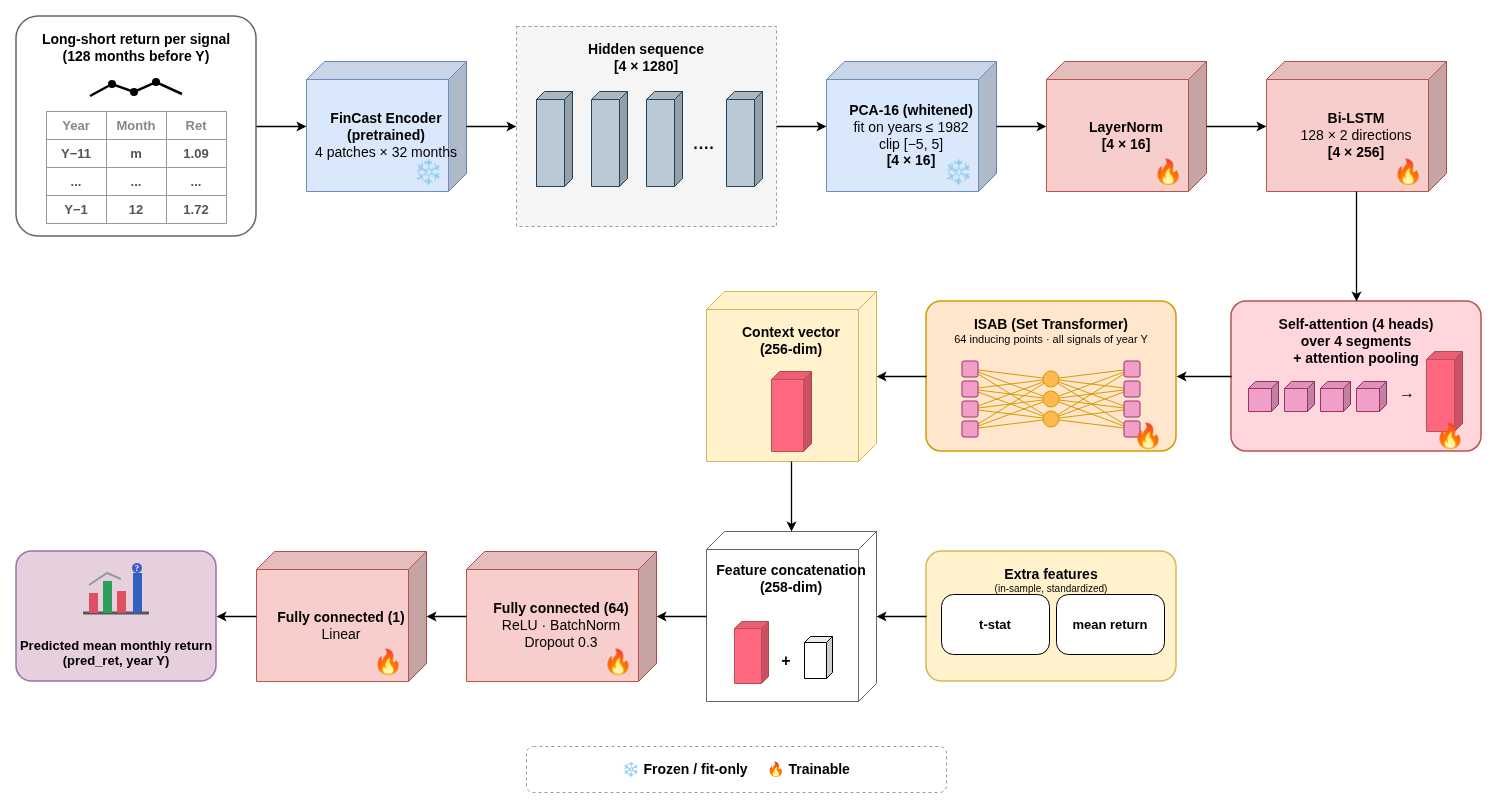
\includegraphics[scale=0.3]{images/final_model.png}
    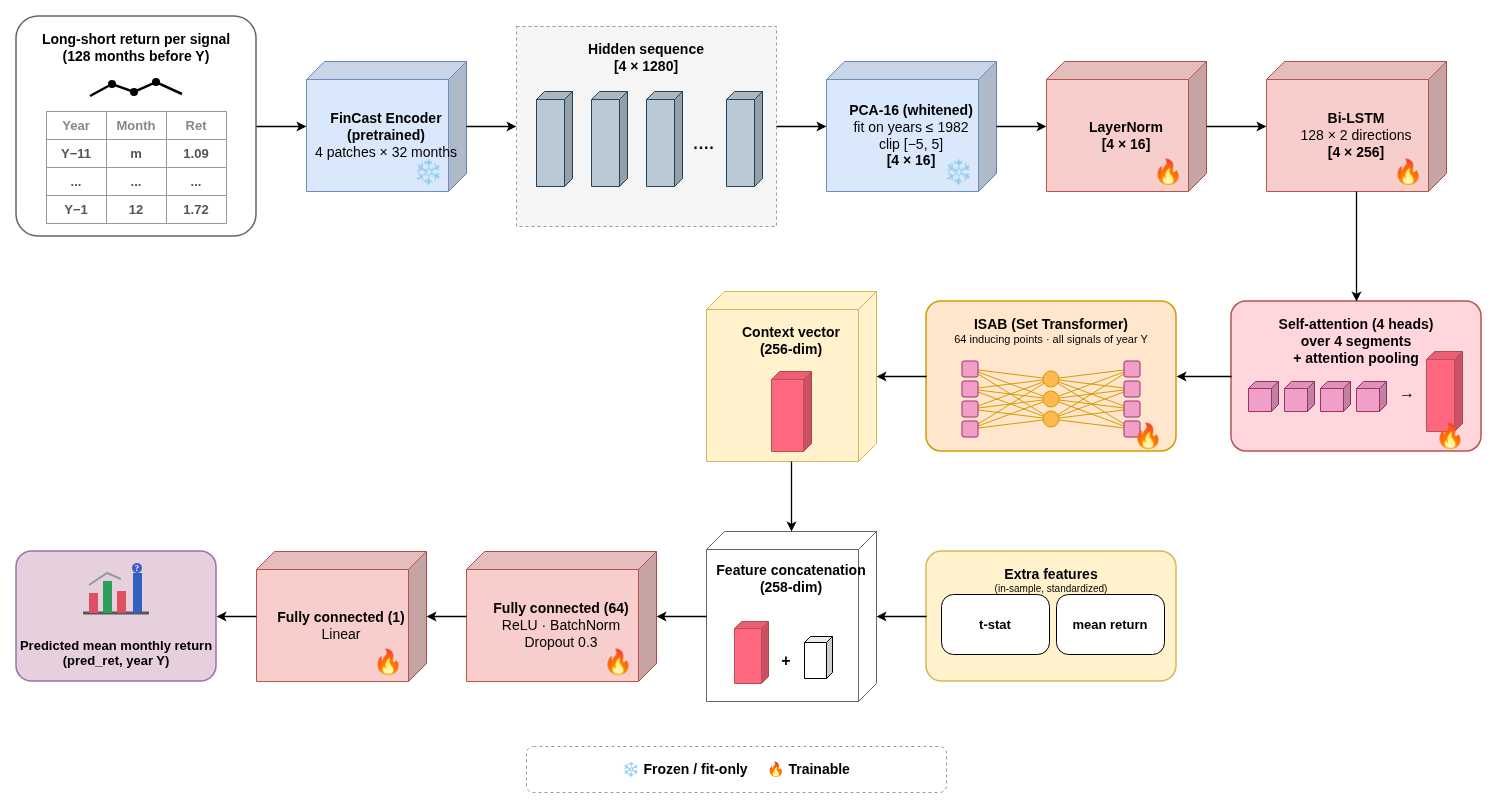
\includegraphics[width=\textwidth]{images/final_model.png}

    \caption{Proposed model}
    \label{fig:Proposed model}
    \end{center}
    \end{figure}
\end{center}
% \subsection{Problem formulation}\label{subsec2}

% % \subsubsection{This is an example for third level head---subsubsection head}\label{subsubsec2}

% % Sample body text. Sample body text. Sample body text. Sample body text. Sample body text. Sample body text. Sample body text. Sample body text. 
% The study focuses on predicting mean long-short returns depending on strategies of accounting ratio, past returns and tickers. The dataset includes signals to build strategies, time, and long-short returns.

% We define $\mathcal{I} = \{1, \ldots, N\}$ as a set of signals from strategies. Each $i \in \mathcal{I}$ is a unique signal. For each $i$, the long-short return sequences are observed monthly. We use the terms ``signal'' and ``strategy'' interchangeably throughout this paper, both referring to a unique long-short trading rule indexed by $i \in \mathcal{I}$ (identified by `signalid` in our dataset).

% \begin{equation} \label{eq:few-shot task}
% {r_i=(r_{i,1},r_{i,2},…,r_{i,T}) \in R^T,}
% \end{equation}

% In which, $r_{i, t}$ denotes the long–short return of signal $i$ in month $t$, generated by an investment strategy that simultaneously takes long positions in assets expected to increase in value and short positions in assets expected to decrease in value. In this setting, the return series $r_i$ serves as the sole input representing signal $i$, without explicitly identifying the underlying industry or ticker. This allows the model to learn generalizable characteristics of investment strategies rather than overfitting to specific assets. Such a representation is particularly suitable for high-throughput signal search.

% In addition, each strategy is characterized by an in-sample summary statistic vector:
% \begin{equation}
% \begin{aligned}
% e_i &= (\tau_i, \bar{r}_i) \in \mathbb{R}^2,\\
% \bar{r}_i &= \frac{1}{T}\sum_{t=1}^{T} r_{i,t},\\
% \tau_i &= \frac{\bar{r}_i}{\hat{\sigma}_i / \sqrt{T}}.
% \end{aligned}
% \label{eq:summary_statistics}
% \end{equation}

% Here, $\hat{\sigma}_i$ denotes the sample standard deviation of the long-short return series $r_i$, and $tau_i$ is the in-sample t-statistic — a criterion commonly used to evaluate and select investment strategies in the empirical asset pricing literature.

% For each strategy i, the out-of-sample (OOS) target variable is defined as the mean return realized over the subsequent evaluation window of length H, which is temporally non-overlapping with the in-sample (IS) window: 

% \begin{equation}
% y_i = \frac{1}{H}\sum_{t=T+1}^{T+H} r_{i,t}
% \label{eq:target}
% \end{equation}

% This strict temporal separation between the IS window ${1, \ldots, T}$, used to construct the model input, and the OOS window $\mathcal{T} = \{T+1, \ldots, T+H\}$, used to construct the prediction target, is designed to avoid look-ahead bias at the strategy level — ensuring that the model is evaluated only on genuinely unseen future performance rather than information already embedded in the input sequence.

% The problem is formulated as a supervised regression task: given the in-sample (IS) return sequence $r_i$ and the auxiliary summary statistics $e_i$, the goal is to learn a mapping function:

% \[
% g_{\theta}: (r_i, e_i) \mapsto \hat{y}_i \in \mathbb{R}
% \]

% ${\theta}$ is parameterized, such that $\hat{y}_i$ provides an accurate prediction of the true out-of-sample target $y_i$.

% The model is trained to minimize the following loss function:
% \begin{equation}
% L_{\text{train}}(\theta)
% =
% \frac{1}{|\mathcal{I}_{\text{train}}|}
% \sum_{i \in \mathcal{I}_{\text{train}}}
% (\hat{y}_i - y_i)^2
% \label{eq:train_loss}
% \end{equation}
% while model selection across training epochs is based on a separate criterion:
% \begin{equation}
% \theta^*
% =
% \underset{\theta^{(e)},\, e=1,\ldots,E}{\arg\max}
% \; \mathrm{IC}_{\mathrm{val}}\!\left(\theta^{(e)}\right),
% \qquad
% \mathrm{IC}_{\mathrm{val}}
% =
% \operatorname{SpearmanCorr}
% \left(
% \hat{\mathbf{y}}^{\mathrm{val}},
% \mathbf{y}^{\mathrm{val}}
% \right).
% \label{eq:model_selection}
% \end{equation}

% where $\theta^{(e)}$ denotes the model parameters at epoch \textit{e}. This separation between the loss used for gradient-based optimization (MSE — smooth and differentiable) and the criterion used for model selection (IC — non-differentiable, but more directly aligned with the true economic objective of ranking strategies) is a common design choice when the true objective of interest — ranking quality — is difficult to optimize directly via gradient descent.

\subsection{Problem formulation}\label{subsec2}

Can a model tell, using only information available in real time, which long-short strategies will earn returns in the future? We study this question using equal-weighted accounting strategies. Published strategies are selected with knowledge of return patterns that occurred in the sample, so their performance contains look-ahead bias \cite{chen2025highthroughputassetpricing}. Thus, for each forecasting year $Y \in \{1983, \ldots, 2020\}$, this study aims to predict the out-of-sample mean return of each strategy in $Y$, using only data before $Y$. This is the quantity that empirical Bayes (EB) predicts, so the two approaches are directly comparable. The difficulty is that in-sample returns are a noisy measure of true performance, because selecting large in-sample returns also selects large sampling error. EB addresses this bias using summary statistics such as the t-stat, and therefore does not explicitly model how returns are distributed over time, although two strategies with the same t-stat can differ in this respect. We hypothesize that the return history itself carries additional information about future performance, and we aim to investigate this possibility.

Let $\mathcal{I}_Y = \{1, \ldots, N_Y\}$ be the set of signals with sufficient history in year $Y$. Each $i \in \mathcal{I}_Y$ is a unique signal, and we use the terms ``signal'' and ``strategy'' interchangeably throughout this paper, both referring to a unique long-short trading rule (identified by \texttt{signalid} in our dataset). The long-short return of signal $i$ in month $t$ is $r_{i,t}$, generated by a strategy that simultaneously takes long positions in assets expected to increase in value and short positions in assets expected to decrease in value. Let month $T$ be the last month before $Y$, and $H = 12$ the number of months in $Y$. Over the $n = 240$ months up to $T$, we compute the in-sample mean return $\bar{r}_i$ and the t-stat $\tau_i$,
\begin{equation}
\bar{r}_i = \frac{1}{n}\sum_{t=T-n+1}^{T} r_{i,t},
\qquad
\tau_i = \frac{\bar{r}_i}{\hat{\sigma}_i / \sqrt{n}},
\label{eq:summary_statistics}
\end{equation}
where $\hat{\sigma}_i$ is the sample standard deviation of $r_{i,t}$ over the same window. Similar to \cite{chen2025highthroughputassetpricing}, who sign strategies to have positive predicted returns, we sign strategies to have a positive in-sample mean, that is, we replace $r_{i,t}$ by $d_i r_{i,t}$ with $d_i = \mathrm{sign}(\bar{r}_i)$. This enables the model to focus on the persistence of performance rather than on its sign.

The input of strategy $i$ consists of two parts. The first is its return sequence over the most recent $T' = 128$ months, $x_i = (r_{i,T-T'+1}, \ldots, r_{i,T}) \in \mathbb{R}^{T'}$. The return series is the sole input representing signal $i$, without identifying the underlying industry or ticker. This design aims to let the model learn generalizable characteristics of strategies rather than overfit to specific assets, and it is consistent with the finding that ticker strategies carry no predictability \cite{chen2025highthroughputassetpricing}. The second part is $e_i = (\tau_i, \bar{r}_i) \in \mathbb{R}^2$, the t-stat on which EB bases its predictions, together with the in-sample mean return. The output is the mean return realized in year $Y$,
\begin{equation}
y_i = \frac{1}{H}\sum_{t=T+1}^{T+H} r_{i,t}.
\label{eq:target}
\end{equation}
The input window ends before the target window begins. This strict temporal separation is designed to avoid look-ahead bias at the strategy level and to ensure that the model is evaluated only on genuinely unseen performance. We do not train on $y_i$ directly. Instead, we express returns in Sharpe ratio units, $S_i = y_i / \hat{\sigma}_i$, and remove the parts that are already known. Let $\bar{S}_Y$ be the mean of $S_j$ over $\mathcal{I}_Y$, which captures good and bad years common to all strategies, and let $z_i$ be the absolute t-stat standardized within year $Y$. The training label is
\begin{equation}
\tilde{y}_i = \mathrm{clip}\!\left(S_i - \bar{S}_Y - b\, z_i;\; q_{1}, q_{99}\right),
\label{eq:label}
\end{equation}
where $b\, z_i$ is the part of future performance that the absolute t-stat already explains, estimated by ridge regression on the 15 years before $Y$, and $q_1$ and $q_{99}$ are the 1st and 99th percentiles of the training residuals. In essence, the model is designed to learn what the t-stat does not already explain. The forecast adds these parts back, $\hat{y}_i = \hat{\sigma}_i(\hat{e}_i + b\, z_i + L_Y)$, where $\hat{e}_i$ is the model output and $L_Y$, the mean of $S_j$ over all years up to $Y-1$, replaces $\bar{S}_Y$ because $\bar{S}_Y$ is unknown in real time.

The problem is a supervised regression task. For each year $Y$, we learn a function $f_{\theta}$ that maps the inputs of all strategies in $\mathcal{I}_Y$ to a prediction $\hat{e}_i$ for each strategy,
\[
f_{\theta}: \left(x_i, e_i;\, \mathcal{X}_Y\right) \mapsto \hat{e}_i \in \mathbb{R},
\qquad
\mathcal{X}_Y = \left\{(x_j, e_j)\right\}_{j \in \mathcal{I}_Y}.
\]
Selecting strategies is a cross-sectional problem, because a strategy is chosen only if its forecast is high relative to the roughly 26,000 other strategies of the same year. Thus, $f_{\theta}$ conditions on the whole set $\mathcal{X}_Y$. We minimize a weighted Huber loss,
\begin{equation}
L(\theta) = \frac{1}{\sum_{Y'} w_{Y'} |\mathcal{I}_{Y'}|}\sum_{Y'} w_{Y'} \sum_{i \in \mathcal{I}_{Y'}} \rho_{\delta}\!\left(\hat{e}_i - \tilde{y}_i\right),
\label{eq:train_loss}
\end{equation}
where $\rho_\delta$ is the Huber loss with $\delta = 1$, and $w_{Y'}$ is a year weight that increases with the mean squared label of year $Y'$. With tens of thousands of strategies, a few extreme returns and a few volatile years would dominate a squared-error loss, and the Huber loss and the year weights are intended to limit these effects. To forecast year $Y$, we train on years up to $Y-2$, validate on year $Y-1$, and re-estimate the model every year, as in the annual refitting of \cite{gu2020empirical}. The loss is only a training device. Following \cite{chen2025highthroughputassetpricing}, we evaluate forecasts through portfolios that equally weight the top $X\%$ of strategies ranked by predicted Sharpe ratios, with $X = 1, 5, 10$, and through the yearly rank correlation between forecasts and realized returns. Portfolio returns never enter the loss, so these evaluations remain out-of-sample.

Several constraints and assumptions make the problem valid. First, everything used for year $Y$ is known before $Y$: returns, $d_i$, $b$, $L_Y$, the clipping bounds, and normalization statistics, which are computed on training years only. The targets of year $Y$ are never used in training or model selection. Second, we do not assume that the relation between past returns and future performance is stable. Indeed, predictability is concentrated before 2004 \cite{chen2025highthroughputassetpricing}, and re-estimating the model every year allows the relation to change. Third, we assume that the in-sample sign is informative about direction, but not that it persists. Strategies whose sign reverses have negative targets, and the model must learn to recognize them. Fourth, EB predictions are never inputs, anchors or parts of the label, and EB serves only as a benchmark. Finally, returns are measured before transaction costs.





% \subsection{Proposed model}\label{subsec3}
% \subsubsection{Overall procedure}\label{subsubModel1}
% The model architecture is illustrated in Figure \ref{fig:Proposed model}. The proposed model leverages the pretrained FinCast model, trained on over 20 billion time points across financial and non-financial domains with various temporal frequencies. FinCast is used solely as a frozen encoder to extract temporal representations from historical long-short returns. These representations are then processed by a Bi-LSTM and learnable attention mechanism, combined with signal-level features (t-statistic and mean IS return), and fed into fully connected layers to predict the mean OOS return.
% \subsubsection{FinCast Embedding Block}\label{subsubModel2}
% In this study, FinCast is employed as a pretrained encoder to extract meaningful latent representations from historical long-short return series. We use the encoder to transform the input time series into a sequence of hidden representations, which is subsequently used as the input to our downstream Bi-LSTM and attention-based prediction module.

% The FinCast block used in this work is as follows:

% \begin{itemize}
% \item \textit{A}: Input preprocessing, patching, and learnable frequency embedding:
% The input time series is first divided into patches. The patched input is then instance-normalized to reduce variations in the scale of individual time series. The normalized patches are subsequently processed by a residual MLP and combined with a learnable frequency embedding. The frequency embedding enables the model to learn information associated with different temporal resolutions, such as seconds, minutes, days, weeks, and months. As a result, the model can distinguish the temporal frequency of different input time series.
% \item \textit{B}: Causal attention with future masking: Each patched token is decomposed into Query, Key, and Value representations, which are used to calculate the attention scores. A causal mask is applied to the attention scores to prevent information from future time steps from being accessed. Specifically, each patch can only attend to the current patch and the patches preceding it, thereby preserving the causal structure of the time series.
% \item \textit{C}: Sparse Mixture-of-Experts (MoE): After the attention stage, each token is routed through a sparse Mixture-of-Experts module using a learnable router. In this module, two experts are selected from four available experts (E1–E4) to process each token. This sparse routing mechanism increases the model capacity without proportionally increasing the computational cost, since only a subset of the available experts is activated for each token.
% \end{itemize}

% The causal attention and sparse MoE blocks are repeatedly stacked times, forming the main stacked decoder of the original FinCast architecture. These blocks account for a substantial portion of the model's parameters and computational capacity and are responsible for learning rich temporal representations from the input time series.
% The original FinCast architecture also contains two additional components: D. the output block and E. the point-quantile loss. The output block consists of a residual MLP and reverse normalization, which are used to transform the model representation back to the original scale of the input data. The point-quantile loss is used to support point and quantile prediction.

% In our framework, however, the output block and point-quantile prediction objective are not used for the downstream prediction task. Instead, we use the pretrained FinCast encoder to extract its hidden representations. Specifically, the hidden sequence generated by the stacked FinCast layers is retained as a compact representation of the historical return dynamics. For each input signal, this representation has a dimension of, corresponding to four latent patches with a hidden dimension of 1280.

% These extracted hidden representations are then passed to our downstream Bi-LSTM with attention pooling, together with the additional in-sample features, to predict the future mean out-of-sample return.

% \subsubsection{LSTM and Attention Block}\label{subsubModel3}

% The obtained hidden sequence from FinCast encoder has the shape of (4, 1280), corresponding to 4 patches with 1280 dimensions per patch. This sequence is subsequently passed into an additional processing block consisting of two main components: A Bidirectional Long Short-Term Memory (Bi-LSTM) network and a learnable Attention Pooling mechanism. This design allows the model to learn additional information between sequences and capture latent temporal dependencies within the representation sequence. After that, the output is a single feature vector, which is used for the downstream prediction task.

% Specifically, the Bi-LSTM is employed to thoroughly model the temporal structure embedded in the return time-series representation. The configuration has a layer of Bi-LSTM that is able to process the sequence of four patches in both forward and backward directions. Therefore, the model captures both historical context and the directional trends across the entire time window. 

% Subsequently, in order to highlight the most insightful components within the LSTM output sequence, we apply an attention mechanism consisting of linear layers: a projection layer combined with a non-linear activation function to transform the LSTM output, and a scoring layer that computes an attention score for each position in the sequence. These scores are then normalized via a softmax function to produce attention weights, reflecting the relative contribution of each patch. This attention mechanism not only helps the model to learn automatically adaptive weights, but it also emphasizes the time segments that carry more predictive signal. 

% The output of the layers above is a 256-dimensional context vector, representing the data in the past used to predict in the future. In order to provide more information for the prediction process, features of t-statistic and mean return from the IS period are aggregated with the 256-dimensional context vector. Therefore, the model can leverage both the deep representation learned from FinCast and classical statistical indicators, bringing information from the past. Following this step of concatenation, a vector with 258 dimensions is obtained. Then, this vector is passed through a neural network including two layers: the fully connected layer with 64 units, which is responsible for learning non-linear combinations of the input features; and the second layer with a single output unit, which produces the final predicted value — namely, the predicted out-of-sample return for the corresponding signal. 


\subsection{Proposed model}\label{subsec3}

\subsubsection{Overall architecture}\label{subsubModel1}
The model architecture is illustrated in Figure \ref{fig:Proposed model}. The proposed model integrates pretrained temporal representations with cross-strategy interactions. It reads the return history of each strategy in addition to its summary statistics, and it forecasts each strategy relative to all strategies of the same year. For a strategy $i$ in forecasting year $Y$, the return sequence $x_i \in \mathbb{R}^{128}$ passes through five stages. We employ a pretrained FinCast encoder to map it to four latent patches of dimension 1280, and apply PCA to compress each patch to 16 dimensions. A Bi-LSTM and an attention pooling layer then turn the four patches into one 256-dimensional context vector. We adopt an Induced Set Attention Block (ISAB) to let this vector interact with the context vectors of all other strategies in year $Y$. Finally, the context vector is concatenated with the two summary statistics $e_i$, forming a 258-dimensional vector, and a fully connected head produces the prediction $\hat{e}_i$, which Equation \eqref{eq:label} converts back to a forecast of the mean return. FinCast and PCA are kept fixed, and all remaining blocks are trained. The model uses only the return sequence and the two summary statistics of a strategy, and not its identity, so it does not condition on tickers or on other labels of the underlying assets.


\subsubsection{FinCast-based temporal representation}\label{subsubModel2}
The t-stat summarizes a return history in a single number, and therefore does not reflect whether a strategy earns steadily or earns most of its profit in a few episodes. To exploit the return history itself, we employ FinCast \cite{zhu2025fincast}, a decoder-only foundation model for financial time series that is pretrained on over 20 billion time points across financial and non-financial domains with various temporal frequencies. The FinCast block used in this work consists of three parts. First, the input is divided into patches, instance-normalized to reduce differences in scale, passed through a residual MLP, and combined with a learnable frequency embedding. Second, a causal attention layer lets each patch attend only to itself and to the preceding patches, which preserves the causal structure of the series. Third, a sparse Mixture-of-Experts (MoE) layer routes each token to two of four experts, which increases capacity without a proportional increase in computation. These layers are stacked 50 times with a hidden dimension of 1280 and 16 attention heads. We do not use the output block or the point-quantile loss of the original model. Instead, we keep the hidden sequence produced by the last stacked layer. Each 128-month sequence is split into four patches of 32 months, so the representation is $h_i \in \mathbb{R}^{4 \times 1280}$, with one vector per patch. FinCast is pretrained on external data and kept frozen, so no parameter of the encoder is fitted to our sample.

\subsubsection{PCA-based feature compression}\label{subsubModel3}
The representation $h_i$ contains $4 \times 1280 = 5{,}120$ numbers per strategy, which is large relative to the roughly 26,000 strategies available in each year. A downstream network with so many inputs may fit noise in the training sample. We therefore employ principal component analysis (PCA) \cite{hotelling1933analysis} to compress each patch to $k = 16$ dimensions, with the aim of reducing redundancy and mitigating overfitting,
\begin{equation}
u_{i,j} = \mathrm{clip}\!\left(\Lambda^{-1/2} V^{\top}\!\left(h_{i,j} - \mu\right);\, -5,\, 5\right) \in \mathbb{R}^{16}, \qquad j = 1, \ldots, 4,
\label{eq:pca}
\end{equation}
where $\mu$ is the mean of the patch vectors, $V$ contains the leading 16 principal directions, $\Lambda$ is the diagonal matrix of the corresponding variances, which whitens the components, and clipping at $\pm 5$ limits outliers. The 16 components retain about 66\% of the variance. To avoid look-ahead bias, $\mu$, $V$ and $\Lambda$ are estimated once on a random sample of strategy-year observations up to 1982, before the first forecasting year. PCA is therefore a fixed linear map that is intended to reduce the complexity of the model and the risk of overfitting.

\subsubsection{Cross-strategy interaction via ISAB}\label{subsubModel4}
The 16-dimensional patches are normalized with layer normalization \cite{ba2016layer} and passed to a Bi-LSTM \cite{hochreiter1997long, schuster1997bidirectional} with 128 hidden units per direction, which reads the four patches in both directions and outputs $H_i \in \mathbb{R}^{4 \times 256}$. To highlight the most informative patches, we first let the patches attend to each other with multi-head self-attention \cite{vaswani2017attention} (4 heads) and a residual connection, giving $\tilde{H}_i$. We then score each patch with $a_{i,j} = \mathrm{softmax}_j\!\left(v^{\top}\tanh(W \tilde{h}_{i,j})\right)$ and pool them into a 256-dimensional context vector $c_i = \sum_{j=1}^{4} a_{i,j}\, \tilde{h}_{i,j}$.

So far, each strategy is processed alone. Selecting strategies, however, is a cross-sectional problem, because a strategy is chosen only if it looks attractive relative to the other strategies of the same year. Let $C_Y \in \mathbb{R}^{N_Y \times 256}$ stack the context vectors of all strategies in year $Y$. Full self-attention over $N_Y \approx 26{,}000$ strategies would cost $O(N_Y^2)$, so we adopt the Induced Set Attention Block (ISAB) of the Set Transformer \cite{lee2019set}. ISAB introduces $m = 64$ learnable inducing points $I \in \mathbb{R}^{64 \times 256}$ that first read the whole year, and then each strategy reads these summaries,
\begin{equation}
M_Y = \mathrm{LN}\!\left(I + \mathrm{MHA}(I, C_Y, C_Y)\right), \qquad
C'_Y = \mathrm{LN}\!\left(C_Y + \mathrm{MHA}(C_Y, M_Y, M_Y)\right),
\label{eq:isab}
\end{equation}
followed by a feed-forward layer with a residual connection and layer normalization, where $\mathrm{MHA}$ denotes multi-head attention with 4 heads and $\mathrm{LN}$ layer normalization. The cost is $O(N_Y m)$. In essence, the inducing points act as 64 learned summaries of the year, and each strategy is placed relative to them. Because all information about the other strategies passes through these 64 summaries, this bottleneck may also make it harder for the model to memorize individual strategies. The output $c'_i$ keeps the dimension 256.

\subsubsection{Prediction head and robust learning objective}\label{subsubModel5}
The vector $c'_i$ is concatenated with the standardized summary statistics $e_i = (\tau_i, \bar{r}_i)$, whose mean and standard deviation are computed on the training years. This enables the model to use both the learned representation and the classical indicators. The resulting 258-dimensional vector $z_i$ passes through a fully connected head,
\begin{equation}
\hat{e}_i = W_2\, \mathrm{Dropout}\!\left(\mathrm{BN}\!\left(\mathrm{ReLU}(W_1 z_i + b_1)\right)\right) + b_2,
\label{eq:head}
\end{equation}
with 64 hidden units, batch normalization \cite{ioffe2015batch} and a dropout rate of 0.3 \cite{srivastava2014dropout}, followed by a single linear output. The output is centered within each year, because the label of Equation \eqref{eq:label} is already centered by $\bar{S}_Y$, and the final forecast follows from $\hat{y}_i = \hat{\sigma}_i(\hat{e}_i + b\, z_i + L_Y)$.

The parameters are trained by minimizing the weighted Huber loss in Equation \eqref{eq:train_loss}, whose two components are designed to address two specific problems. First, a small number of strategies have extreme returns, which would dominate a squared-error loss. The Huber loss \cite{huber1964robust} is quadratic for small errors and linear for large ones, which limits their influence. Second, some years carry much more information than others. We adapt the idea of loss-weighted gradient scaling in \cite{holen2024loss}, where more informative episodes receive more weight, by treating each forecasting year as an episode and setting
\begin{equation}
w_{Y'} \propto \frac{1}{2}\left(1 + \frac{v_{Y'}}{\bar{v}}\right),
\label{eq:year_weight}
\end{equation}
where $v_{Y'}$ is the mean squared label in year $Y'$, $\bar{v}$ is its average over training years, and the weights are normalized to average one. Years with more variation in the label then receive more weight, but no year is ignored. We optimize with AdamW \cite{loshchilov2019decoupled} (learning rate $10^{-3}$, weight decay $10^{-2}$), clip gradients at norm one, and use the whole cross-section of one year as a single update. For each forecasting year, training starts from the weights of the previous year and runs for at most three epochs, and the epoch with the lowest validation loss on year $Y-1$ is kept.

 % Data
% \section{Data}\label{sec4}
% The trading strategy universe used in this study is identical to that of the high-throughput asset pricing framework of Chen et al \cite{chen2025highthroughputassetpricing}. However, since Chen et al. demonstrate that ticker-level identifying information contributes little explanatory power to their results, we deliberately restrict our input space to strategies constructed purely from accounting ratios and past returns, discarding any ticker-specific features. This choice keeps our model's input strictly return-based and asset-agnostic, consistent with the high-throughput screening philosophy of treating each strategy as an anonymous, interchangeable unit of evaluation.

% \textbf{Accounting ratio strategies ($\approx 60,000$):} Following the design of \citet{yan2017fundamental}, \citet{chen2025highthroughputassetpricing} construct approximately 30,000 accounting-ratio signals as follows. Let $X$ denote one of 240 accounting variables sourced from Compustat (augmented with CRSP market equity), and let $Y$ denote one of 65 variables among these 240 that is strictly positive for at least 25\% of firms as of 1963. Two transformations are applied to each $(X, Y)$ pair — the level ratio X/Y and the first-difference ratio $\Delta X / \mathrm{lag}(Y)$ — yielding $240 \times 65 \times 2 \approx 30{,}000$ candidate signals. Each signal is then used to form both equal-weighted and value-weighted long-short decile portfolios, doubling the count to approximately 60,000 accounting-based strategies. These strategies were obtained from Andrew Chen's public data repository; we thank the authors for making this dataset available.

% \textbf{Past-return-based strategies ($\approx 38,000$)}. Also inspired by \citet{yan2017fundamental}, past-return strategies are constructed by selecting 4 quarters out of the trailing 20 quarters and computing the first four central moments (mean, variance, skewness, kurtosis) of returns within the selected quarters, yielding $\binom{20}{4} \times 4 = 19{,}380 \text{ signals}$. To this set, the raw return was added in each of the past 20 individual quarters, as well as the mean return over the trailing 2 and 3 quarters, contributing 20+2=22 additional signals — for a total of 19,380 + 22 = 19,402 signals. As with the accounting-based signals, each is used to construct both equal-weighted and value-weighted long-short decile strategies, doubling the total to approximately 38,000 past-return-based strategies.

\section{Experiments}\label{sec4}

This section describes the data and the experimental design, and examines the accuracy of the forecasts. Section \ref{sec5} then evaluates the portfolios that each method selects.

\subsection{Data}\label{subsec4_1}

\subsubsection{Dataset}
We use the long-short strategies of \cite{chen2025highthroughputassetpricing}: 136,192 strategies in six families, formed from three data sources (accounting ratios, past returns and tickers) and two weighting schemes (equal- and value-weighted). Since ticker strategies carry no predictability and 91.0\% of the top 1\% selected by empirical Bayes (EB) are equal-weighted accounting strategies \cite{chen2025highthroughputassetpricing}, we focus on the equal-weighted accounting family (29,314 strategies). Following \citet{yan2017fundamental}, they are built from about 30,000 signals of the form $X/Y$ and $\Delta X/\mathrm{lag}(Y)$, with $X$ one of 240 Compustat variables and $Y$ one of 65 variables. The strategies come from the public repository of Andrew Chen, and they are generated by systematic search rather than selected for notable returns. As a noise control in Section \ref{subsec5_2}, we also form a pool that adds the equal-weighted ticker strategies, which make up 43.5\% of the pooled strategies.

\subsubsection{Sample construction and data splitting}
For each forecasting year $Y$, we keep strategies with at least 36 months of returns in the 20 years before $Y$, which leaves about 25,600 strategies per year. The resulting table has 1,189,707 strategy-year observations from 1966 to 2020, and the first forecasting year is 1983. Training, validation and testing follow Section \ref{subsec2}, with at most the 500,000 most recent observations used for training. We divide the 38 forecasting years into a development period (1983--2004) and a holdout period (2005--2020), following the 2004 break documented by \cite{chen2025highthroughputassetpricing}. The architecture, hyperparameters and the selected model are chosen on the development period only, and the holdout period, which is out of sample for all choices, is used only for reporting.

\subsection{Analysis and results}\label{subsec4_2}

\subsubsection{Implementation details}
We use the pretrained FinCast weights of \cite{zhu2025fincast} (50 layers, 16 heads, hidden dimension 1280, sparse Mixture-of-Experts), without fine-tuning. Together with the components of Section \ref{subsec3}, the proposed model has 1,565,857 trainable parameters. We train six seeds and select the one with the highest mean Sharpe ratio over 1995--2004. Because GPU computation is not deterministic, we store the weights of the selected model for every year, and all main results in Section \ref{sec5} are computed from these stored weights. Experiments run on one NVIDIA RTX 5060 Ti GPU with PyTorch 2.11.

\subsubsection{Baseline methods}
All methods select from the same family and years, and differ only in the forecast used for ranking. \textit{EB mining} reproduces \cite{chen2025highthroughputassetpricing}, fitting a mixture of two normals to the t-stats with the past 20 years of returns. \textit{Naive mining} ranks strategies by the absolute in-sample t-stat. The \textit{baseline model} uses FinCast, a Bi-LSTM and attention pooling with the in-sample t-stat and mean return, trained with a squared-error loss to predict the mean return, without sign orientation, PCA or ISAB (average forecast of three runs).

\subsubsection{Evaluation metrics}
We evaluate the methods at two levels. At the forecast level, we report the information coefficient (IC), the average yearly Spearman correlation between forecasts and realized returns, and a calibration slope across 20 groups ranked by forecast (one indicates unbiased forecasts). At the portfolio level, we apply the rule of Section \ref{subsec2}, following \cite{chen2025highthroughputassetpricing}: each year we sign strategies by their forecasts, rank them by predicted Sharpe ratio (forecast divided by in-sample standard deviation), and hold the equal-weighted top $X\%$ for the 12 months of the year. We report the mean return (percent per year), the t-stat and the annualized Sharpe ratio, computed over all months of a period and before transaction costs. Sharpe ratio differences are tested with the HAC test of \cite{ledoit2008robust} (12 lags) and, as a check, with a block bootstrap by year.

\subsubsection{Forecast accuracy}
We first ask how accurately each method forecasts the mean return of all strategies, and in Section \ref{sec5} how well it selects the best ones. The two questions differ, because a method can rank the top of the list well and still estimate the level of returns less precisely. Table \ref{tab:forecast} shows that EB mining has a higher IC in the development period (0.188 against 0.151, $p = 0.013$), while the ICs are not significantly different in the holdout period (0.021 against 0.043, $p = 0.49$) and the full period (0.118 against 0.106, $p = 0.52$). The IC of the proposed model is higher than that of EB mining in the two later subperiods, 2005--2012 (0.055 against 0.020) and 2013--2020 (0.032 against 0.023), when predictability is weaker, and lower in the two earlier ones. The proposed model has a positive IC in 30 of the 38 years against 28 for EB mining, and the dispersion of its yearly IC is lower (0.138 against 0.168). The calibration slope of EB mining is closer to one in both periods (0.88 against 0.79 in the development period, and 0.31 against 0.19 in the holdout period), so EB shrinkage estimates the magnitude of expected returns more accurately. Thus, EB mining is the more precise estimator of expected returns, while the proposed model ranks strategies with comparable accuracy and more stability across years. The portfolio tests of Section \ref{sec5} show which of these properties matters for selecting strategies.

\begin{table}[h]
\caption{Forecast accuracy over all strategies. IC is the mean yearly Spearman correlation; the calibration slope is computed across 20 groups of forecasts (one indicates unbiased forecasts).}\label{tab:forecast}%
\small
\begin{tabular}{@{}llccc@{}}
\toprule
Measure & Method & Development & Holdout & Full \\
\midrule
IC & EB mining & 0.188 & 0.021 & 0.118 \\
 & Proposed model & 0.151 & 0.043 & 0.106 \\
Years with positive IC & EB mining & 20 of 22 & 8 of 16 & 28 of 38 \\
 & Proposed model & 19 of 22 & 11 of 16 & 30 of 38 \\
Calibration slope & EB mining & 0.88 & 0.31 & -- \\
 & Proposed model & 0.79 & 0.19 & -- \\
\botrule
\end{tabular}
\end{table}

\subsection{Ablation study}\label{subsec4_3}
We replace one component of the final configuration at a time and train each configuration three times, because retraining is not deterministic. Table \ref{tab:ablation} reports the mean Sharpe ratio over the top 1\%, 5\% and 10\% portfolios and the difference from the reference (the final configuration retrained in the same way). The run-to-run standard deviation of the reference is 0.03 in the development period and 0.13 in the holdout period, so we regard a difference as meaningful only when it clearly exceeds this variation. We report the components that show such a difference, and state the outcome for the others at the end.

\begin{table}[h]
\caption{Ablation of the pretrained encoder and the PCA compression. Values are Sharpe ratios averaged over the top 1\%, 5\% and 10\% portfolios and over three runs. $\Delta$ is the difference from the reference.}\label{tab:ablation}%
\small
\begin{tabular}{@{}lcccc@{}}
\toprule
Configuration & Development & Holdout & $\Delta$ Dev. & $\Delta$ Hold. \\
\midrule
Random-initialized FinCast (no pretraining) & 1.80 & 0.66 & $-0.04$ & $-0.18$ \\
PCA with 8 components & 1.95 & 0.67 & $+0.10$ & $-0.17$ \\
PCA with 32 components & 1.85 & 0.77 & $0.00$ & $-0.07$ \\
PCA with 64 components & 1.64 & 0.74 & $-0.20$ & $-0.10$ \\
\midrule
Reference (final configuration, retrained) & 1.85 & 0.84 & -- & -- \\
\botrule
\end{tabular}
\end{table}

\subsubsection{FinCast contribution}
Replacing the pretrained encoder with the same architecture at random initialization gives the lowest holdout Sharpe ratio of all variants (0.66 against 0.84), a difference larger than the run-to-run variation. This suggests that the pretrained temporal representations contribute to the performance after 2004. Other pretrained encoders tested during development (Chronos-2, EXAONE, Sundial) did not exceed FinCast.

\subsubsection{PCA contribution}
With 8 components the development Sharpe ratio rises ($+0.10$) but the holdout one falls ($-0.17$), a pattern typical of fitting the development period too closely, and with 64 components both fall. The 16-dimensional compression gives the best balance between the two periods among the sizes we tested, consistent with the aim of reducing redundancy and mitigating overfitting. We did not test a model without compression.

\subsubsection{Label construction contribution}
During development, adding the Sharpe label centered by the year mean (Equation \eqref{eq:label}) to a model without it raised the Sharpe ratio from 1.37 to 1.84 in the development period and from 0.69 to 0.81 in the holdout period, well beyond the variation between runs and the largest improvement in our experiments. A possible explanation is that selecting the top of the ranking depends on comparing strategies within a year, and the label carries this comparison directly. This result comes from the stepwise development and not from the three-run protocol of Table \ref{tab:ablation}.

\subsubsection{Other components}
We also removed or replaced ISAB, the Huber loss, the year weights and the $|t|$ baseline in the label. For each of them, the three-run mean stays within the run-to-run variation of the reference, so we do not claim a distinguishable contribution and keep them as design choices. For ISAB, an inspection of the trained model suggests that it acts mainly as an additional transformation of each strategy, since the summaries of its inducing points differ by only 2--3\% between years.


% Result
% \section{Results}\label{sec5}

% We compare four signal-selection methods: Empirical Bayes (EB) Mining, Naive Mining, LSTM + Attention, and FinCast + LSTM + Attention.
% \begin{enumerate}
% \item \textbf{Empirical Bayes (EB) Mining}: We reproduce the results obtained by applying the EB procedure of Chen et al. \cite{chen2025highthroughputassetpricing}.
% \item \textbf{Naive Mining}: We follow the approach used by Chen et al. \cite{chen2025highthroughputassetpricing} in their high-throughput experiments, where signals are selected based on their in-sample t-statistics.
% \item \textbf{LSTM + Attention}: This method uses only a bidirectional LSTM and an attention mechanism to predict future returns from the input signals.
% \item \textbf{FinCast + LSTM + Attention}: This is the proposed method, which incorporates representations learned by FinCast into the LSTM + Attention architecture for return prediction and signal selection.
% \end{enumerate}
% Table \ref{tab1} presents the comparison of the four signal-selection methods-Empirical Bayes (EB) Mining, Naive Mining, LSTM + Attention, and FinCast + LSTM + Attention-across the four signal families: DataMinedLongShortReturnsEW/VW and PastReturnSignalsLongShortEW/VW.

% When evaluated on the full signal universe, LSTM + Attention achieves the highest Sharpe ratios at Top 1\% and Top 10\%, with Sharpe ratios of 1.93 and 2.39, respectively. At Top 5\%, however, EB Mining performs slightly better, achieving a Sharpe ratio of 2.31 compared with 2.04 for LSTM + Attention. In contrast, FinCast + LSTM + Attention performs substantially worse on the full signal universe, with Sharpe ratios of only 0.01, 0.89, and 1.01 at Top 1\%, Top 5\%, and Top 10\%, respectively.

% These results do not support our initial hypothesis that the deep representations learned by FinCast would consistently improve signal-selection performance over traditional statistical approaches. This unexpected result motivated a more detailed analysis at the signal-family level.

% Table \ref{tab2} reports the results after excluding the DataMinedLongShortReturnsVW family, which was the only family exhibiting a negative rank information coefficient (IC = -0.012) during training. This negative IC suggests that FinCast failed to learn a meaningful predictive relationship for this particular signal family.

% After excluding this problematic family, the performance of FinCast + LSTM + Attention improves substantially and becomes consistently superior across all three selection thresholds. At Top 1\%, the proposed method achieves a Sharpe ratio of 3.24, compared with 0.86 for EB Mining, 0.99 for Naive Mining, and 1.95 for LSTM + Attention. At Top 5\%, it achieves 2.74, compared with 2.19, 1.44, and 1.95, respectively. At Top 10\%, the proposed method achieves 2.53, compared with 2.27, 0.67, and 2.20, respectively.

% These findings highlight the potential of the proposed approach. Once the signal family with unstable predictive behavior is excluded, the representations learned by FinCast, combined with LSTM and attention mechanisms, appear to capture more nuanced predictive structures than the traditional statistical approaches. This also suggests that the effectiveness of the proposed method depends critically on the quality and predictive stability of the underlying signal families.


% % Tables can be inserted via the normal table and tabular environment. To put
% % footnotes inside tables you should use \verb+\footnotetext[]{...}+ tag.
% % The footnote appears just below the table itself (refer Tables~\ref{tab1} and \ref{tab2}). 
% % For the corresponding footnotemark use \verb+\footnotemark[...]+

% \begin{table}[h]
% \caption{Returns of Data-Mined Long-Short Portfolios}\label{tab1}%
% \begin{tabular}{@{}lllll@{}}
% \toprule
% Method & Num Strats Combined & Mean Return (\% ann)  & t-stat & Sharpe Ratio (ann) \\
% \midrule
% EB Mining Top 1\%    & 907 & 1.16  & 0.80 & 0.98 \\
% EB Mining Top 5\%    & 4534   & 1.53  & 1.89   & \textbf{2.31}  \\
% EB Mining Top 10\%    & 9069   & 0.88  & 1.65 & 2.02  \\
% Naive Mining Top 1\%    & 907   & 1.08  & 0.77 & 0.95     \\
% Naive Mining Top 5\%    & 4534   & 0.63  & 0.61  &  0.74   \\
% Naive Mining Top 10\%    & 9069   & 0.01  &  0.01 &  0.01    \\
% LSTM + Attention  Top 1\%    & 907   & 6.61  & 1.58  &   \textbf{1.93}  \\
% LSTM + Attention  Top 5\%    & 4534   & 5.47    &  1.66 & 2.04  \\
% LSTM + Attention  Top 10\%    & 9069   & 5.01  &  1.95  &  \textbf{2.39}   \\
% FinCast + LSTM + Attention Top 1\%    & 907   & 0.01  & 0.01  &   0.01  \\
% FinCast + LSTM + Attention Top 5\%    & 4534   & 0.63    &  0.73 & 0.89  \\
% FinCast + LSTM + Attention Top 10\%    & 9069   & 0.57  &  0.82  &  1.01   \\

% \botrule
% \end{tabular}


% % \footnotetext{Source: This is an example of table footnote. This is an example of table footnote.}
% % \footnotetext[1]{Example for a first table footnote. This is an example of table footnote.}
% % \footnotetext[2]{Example for a second table footnote. This is an example of table footnote.}
% \end{table}


% \begin{table}[h]
% \caption{Returns of Data-Mined Long-Short Portfolios without Accounting VW strategies}\label{tab2}%
% \begin{tabular}{@{}lllll@{}}
% \toprule
% Method & Num Strats Combined & Mean Return (\% ann)  & t-stat & Sharpe Ratio (ann) \\
% \midrule
% EB Mining Top 1\%    & 648 & 1.08  & 0.71 & 0.86  \\
% EB Mining Top 5\%    &  3238   & 1.67  & 1.79   & 2.19  \\
% EB Mining Top 10\%    & 6475   & 1.25  & 1.85 & 2.27  \\
% Naive Mining Top 1\%    & 648   & 1.17  & 0.81 & 0.99    \\
% Naive Mining Top 5\%    & 3238   & 1.17  & 1.18  &  1.44   \\
% Naive Mining Top 10\%    & 6475   & 0.43  &  0.55 &  0.67  \\
% LSTM + Attention 1\%    & 648   & 6.36  &  1.59 &  1.95   \\
% LSTM + Attention 5\%    & 3238   & 5.81 &  1.59 &  1.95   \\
% LSTM + Attention 10\%    & 6475   & 5.25  &  1.79 &  2.20   \\
% FinCast + LSTM + Attention Top 1\%    & 648   & 2.08  & 2.65  &   \textbf{3.24}  \\
% FinCast + LSTM + Attention Top 5\%    & 3238   & 1.72    &  2.24 & \textbf{2.74}  \\
% FinCast + LSTM + Attention Top 10\%    & 6475   & 1.45  &  2.06  &  \textbf{2.53}  \\

% \botrule
% \end{tabular}


% % \footnotetext{Source: This is an example of table footnote. This is an example of table footnote.}
% % \footnotetext[1]{Example for a first table footnote. This is an example of table footnote.}
% % \footnotetext[2]{Example for a second table footnote. This is an example of table footnote.}
% \end{table}




% \begin{table}[h]
% \caption{Family-level summary}\label{tab3}%
% \begin{tabular}{@{}lllll@{}}
% \toprule
% Sinal Family & Training Set Size & Test Set Size & IC & Long-short spread \\
% \midrule
% DataMinedLongShortReturnsEW   & 771580   & 207800 & 0.077529  & 0.243258  \\
% DataMinedLongShortReturnsVW   &  771556  & 207800 & -0.011534  & -0.066170  \\
% PastReturnSignalsLongShort-ew   & 601462  & 155216   & 0.088853 & 0.281985\\
% PastReturnSignalsLongShort-vw   & 601462     & 155216 & 0.045984 & 0.123014   \\

% \botrule
% \end{tabular}


% % \footnotetext{Source: This is an example of table footnote. This is an example of table footnote.}
% % \footnotetext[1]{Example for a first table footnote. This is an example of table footnote.}
% % \footnotetext[2]{Example for a second table footnote. This is an example of table footnote.}
% \end{table}

% Figure \ref{fig:result1} illustrates the cumulative performance of the Top 5\% portfolios over the full four-family signal universe. LSTM + Attention shows the strongest and most consistent performance throughout the sample period, while EB Mining also exhibits a relatively stable upward trend. FinCast + LSTM + Attention, although weaker in the early part of the sample, shows a notable improvement in 2020, indicating that the FinCast-based representation can identify profitable predictive patterns under certain market conditions. However, this improvement is not sustained in 2021, suggesting that its performance is more sensitive to the composition of the underlying signal families. This observation motivates the additional analysis in Table \ref{tab2}, where the problematic signal family is excluded and the performance of the FinCast-based approach improves substantially.
 
% \begin{center}
%     \begin{figure}[h]
%     \begin{center}
%     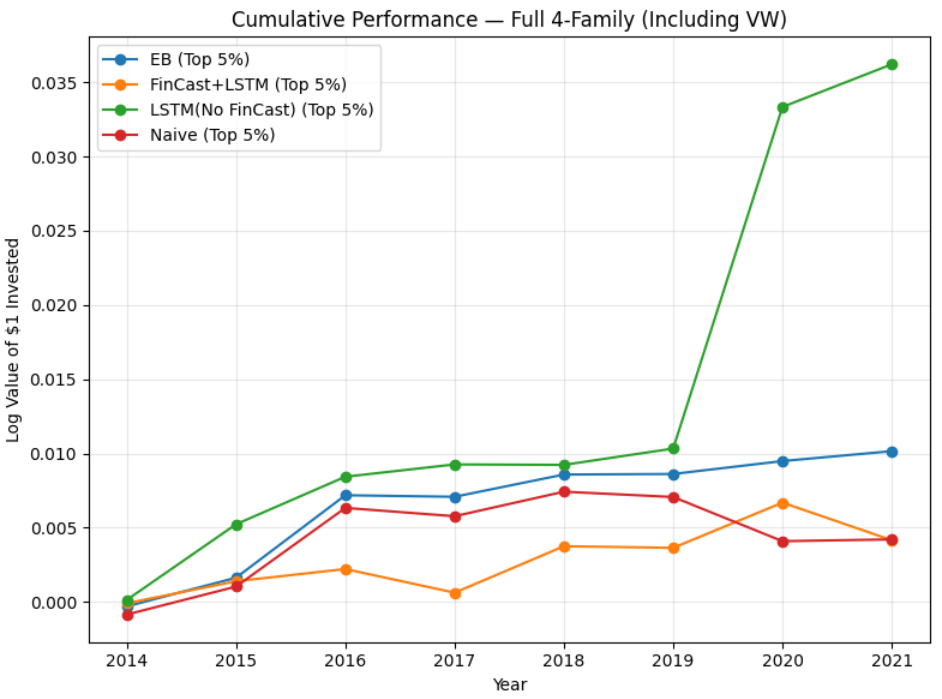
\includegraphics[scale=0.8]{images/result1.png}
%     \caption{Cumulative Out-of-Sample Performance of Top 5\% Portfolios (2014–2021)}
%     \label{fig:result1}
%     \end{center}
%     \end{figure}
% \end{center}

% \begin{center}
%     \begin{figure}[h]
%     \begin{center}
%     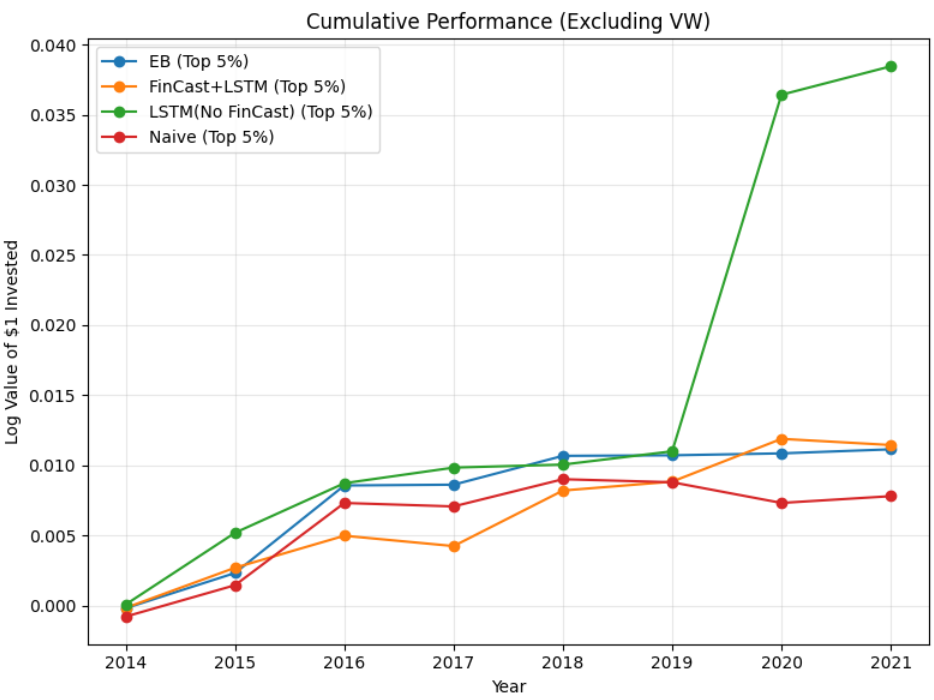
\includegraphics[scale=0.8]{images/result2.png}
%     \caption{Cumulative Out-of-Sample Performance of Top 5\% Portfolios (2014–2021) without Accounting VW strategies}
%     \label{fig:result2}
%     \end{center}
%     \end{figure}
% \end{center}

% \noindent

\section{Results}\label{sec5}

Can the proposed model select better strategies than EB mining using only information available in real time? We answer this question with the portfolio tests of Section \ref{subsec4_2}.

\subsection{Overall performance comparison}\label{subsec5_1}

\subsubsection{Baseline comparison}
Table \ref{tab:sharpe} compares the four methods of Section \ref{subsec4_2}, ordered from the weakest to the proposed model. The baseline model has the lowest Sharpe ratio in every cell, so the improvement of the proposed model comes from the design of Section \ref{subsec3} and not from the FinCast representations alone (for the top 1\%, 1.95 against 1.34 in the development period and 1.11 against 0.61 in the holdout period). Naive mining is the closest competitor of the proposed model: it equals the proposed model for the development top 1\% (1.95) and is higher for the development top 5\% (1.99). The proposed model has the highest Sharpe ratio in all three holdout cells and in the full-period top 1\% and 5\%, and the highest or tied-highest value in 6 of the 9 cells. The exception that favors EB mining is the development top 10\% (1.86 against 1.82).

\begin{table}[h]
\caption{Annualized Sharpe ratios of equal-weighted long-short portfolios from the top 1\%, 5\% and 10\% of equal-weighted accounting strategies. The development period is 1983--2004 and the holdout period is 2005--2020.}\label{tab:sharpe}%
\small
\begin{tabular}{@{}lccccccccc@{}}
\toprule
 & \multicolumn{3}{c}{Development} & \multicolumn{3}{c}{Holdout} & \multicolumn{3}{c}{Full} \\
\cmidrule(lr){2-4}\cmidrule(lr){5-7}\cmidrule(lr){8-10}
Method & 1\% & 5\% & 10\% & 1\% & 5\% & 10\% & 1\% & 5\% & 10\% \\
\midrule
Baseline model & 1.34 & 1.23 & 1.16 & 0.61 & 0.51 & 0.54 & 1.07 & 0.97 & 0.94 \\
Naive mining ($|t|$ rule) & \textbf{1.95} & \textbf{1.99} & 1.85 & 0.84 & 0.75 & 0.83 & 1.52 & 1.51 & 1.47 \\
EB mining & 1.55 & 1.91 & \textbf{1.86} & 0.82 & 0.78 & 0.86 & 1.27 & 1.48 & \textbf{1.48} \\
Proposed model & \textbf{1.95} & 1.95 & 1.82 & \textbf{1.11} & \textbf{0.88} & \textbf{0.88} & \textbf{1.62} & \textbf{1.54} & 1.46 \\
\botrule
\end{tabular}
\end{table}

\subsubsection{Selection performance}
Table \ref{tab:selection} reports returns, t-stats and the significance of the Sharpe ratio differences. The top 1\% portfolio of EB mining earns 8.95\% per year in the development period and 2.79\% in the holdout period, with t-stats of 7.26 and 3.27. The proposed model earns 9.36\% and 3.54\%, with t-stats of 9.15 and 4.45. The Sharpe ratio difference from EB mining is significant in the development ($p = 0.032$), holdout ($p = 0.028$) and full ($p = 0.005$) periods, and a block bootstrap by year gives 0.059, 0.051 and 0.010. Against naive mining, the proposed model is indistinguishable in the development period ($p = 0.97$) and higher in the holdout period ($p = 0.028$). For the top 5\% and 10\%, no difference from EB mining is significant, so the advantage concentrates at the top of the ranking, which matters most to a data miner who buys few strategies.

\begin{table}[h]
\caption{Mean return (percent per year), t-stat, and $p$-values of the Sharpe ratio difference between the proposed model and each method (HAC test).}\label{tab:selection}%
\small
\begin{tabular}{@{}llcccccc@{}}
\toprule
 & & \multicolumn{2}{c}{EB mining} & \multicolumn{2}{c}{Proposed model} & \multicolumn{2}{c}{$p$-value vs.} \\
\cmidrule(lr){3-4}\cmidrule(lr){5-6}\cmidrule(lr){7-8}
Portfolio & Period & Return & t-stat & Return & t-stat & EB & Naive \\
\midrule
Top 1\%  & Development & 8.95 & 7.26 & 9.36 & 9.15 & 0.032 & 0.970 \\
         & Holdout     & 2.79 & 3.27 & 3.54 & 4.45 & 0.028 & 0.028 \\
         & Full        & 6.36 & 7.84 & 6.91 & 9.97 & 0.005 & 0.104 \\
Top 5\%  & Development & 8.42 & 8.97 & 8.05 & 9.16 & 0.625 & 0.445 \\
         & Holdout     & 2.29 & 3.11 & 2.44 & 3.50 & 0.330 & 0.189 \\
         & Full        & 5.84 & 9.11 & 5.69 & 9.46 & 0.317 & 0.646 \\
Top 10\% & Development & 7.73 & 8.74 & 7.13 & 8.51 & 0.315 & 0.459 \\
         & Holdout     & 2.26 & 3.42 & 2.16 & 3.51 & 0.828 & 0.653 \\
         & Full        & 5.43 & 9.11 & 5.04 & 8.98 & 0.626 & 0.838 \\
\botrule
\end{tabular}
\end{table}

\subsubsection{Where the methods disagree}
The proposed model and EB mining share only part of their top 1\% portfolios: averaged over the 38 years, 51.5\% of the strategies in the top 1\% of the proposed model are also in that of EB mining. Table \ref{tab:disagree} separates the strategies selected only by EB mining, by both methods and only by the proposed model (about 122, 130 and 122 strategies per year). The strategies selected only by the proposed model earn a Sharpe ratio of 1.63 over the full period, against 0.85 for those selected only by EB mining, and the difference is significant in the development ($p < 0.001$), holdout ($p = 0.038$) and full ($p < 0.001$) periods. Their mean return is also higher (6.66\% against 5.81\% per year), although this difference alone is not statistically significant ($t = 0.99$), and their t-stat is much higher (10.02 against 5.24), so their advantage lies mainly in more stable returns. Thus, where the two methods disagree, the choices of the proposed model are the better ones. This suggests that the return history carries information about future performance that the summary statistics used by EB mining do not.

\begin{table}[h]
\caption{Top 1\% portfolios split by which method selects the strategy. Mean return is in percent per year.}\label{tab:disagree}%
\small
\begin{tabular}{@{}lccccccccc@{}}
\toprule
 & \multicolumn{3}{c}{Development} & \multicolumn{3}{c}{Holdout} & \multicolumn{3}{c}{Full} \\
\cmidrule(lr){2-4}\cmidrule(lr){5-7}\cmidrule(lr){8-10}
Selected by & Return & t-stat & Sharpe & Return & t-stat & Sharpe & Return & t-stat & Sharpe \\
\midrule
EB mining only & 8.37 & 4.69 & 1.00 & 2.29 & 2.53 & 0.63 & 5.81 & 5.24 & 0.85 \\
Both methods & 9.77 & 8.98 & 1.91 & 3.45 & 3.80 & 0.95 & 7.11 & 9.47 & 1.54 \\
Proposed model only & 8.85 & 9.14 & \textbf{1.95} & 3.65 & 4.56 & \textbf{1.14} & 6.66 & 10.02 & \textbf{1.63} \\
\botrule
\end{tabular}
\end{table}

\subsubsection{Summary of the comparison}
The proposed model selects the top 1\% of strategies with a higher Sharpe ratio, mean return and t-stat than EB mining in the development, holdout and full periods, and the Sharpe ratio differences are statistically significant. In the holdout period, it has the highest Sharpe ratio of the four methods at every portfolio size. The strategies that it selects beyond those of EB mining earn a Sharpe ratio nearly twice as high (1.63 against 0.85). For the top 5\% and 10\%, the methods are statistically indistinguishable. The model also treats ticker strategies, which carry no predictability, as noise at the top of its ranking: they are only 0.19\% of its top 1\% portfolio, although they are 43.5\% of the pool (Section \ref{subsec5_2}).

\subsection{Robustness to noise strategies}\label{subsec5_2}

\subsubsection{Ticker control}
Ticker strategies carry no predictability \cite{chen2025highthroughputassetpricing}, so they provide a control for noise: a method that mistakes noise for signal would select them. We apply the trained model to the pool that adds the equal-weighted ticker strategies, without retraining and without the model having seen ticker strategies. They make up 43.5\% of the pool, so a random selection would hold this share. They are 0.19\%, 3.43\% and 9.30\% of the top 1\%, 5\% and 10\% of the proposed model (Table \ref{tab:ticker}). The 33 ticker strategies in the top 1\% over the 38 years earn $-0.07\%$ per month, which is consistent with noise, and the IC of the model within ticker strategies is close to zero ($-0.035$). Thus, the proposed model recognizes ticker strategies as noise at the top of its ranking.

\subsubsection{Sensitivity analysis}
Table \ref{tab:ticker} compares the methods on the pool that adds ticker strategies with the accounting family alone. Adding a noise family changes the top 1\% Sharpe ratio of the proposed model by $+0.07$ in the development period and $-0.06$ in the holdout period, and that of naive mining by $+0.06$ and $-0.09$. For EB mining, which is re-estimated on the pool, the change is $+0.17$ and $-0.07$. The proposed model has the highest top 1\% Sharpe ratio on the pool in both periods (2.02 and 1.05). Ticker strategies enter the top 5\% and 10\% of the proposed model more often than those of EB mining (Table \ref{tab:ticker}), so EB mining shrinks noise more strongly beyond the top 1\%.

\begin{table}[h]
\caption{Sensitivity to the ticker family. Share of ticker strategies in the top 1\%, 5\% and 10\% portfolios of the pool, and top 1\% Sharpe ratios on the pool and on the accounting family alone.}\label{tab:ticker}%
\small
\begin{tabular}{@{}lccccccc@{}}
\toprule
 & \multicolumn{3}{c}{Ticker share (\%)} & \multicolumn{2}{c}{Sharpe, pool} & \multicolumn{2}{c}{Sharpe, accounting only} \\
\cmidrule(lr){2-4}\cmidrule(lr){5-6}\cmidrule(lr){7-8}
Method & 1\% & 5\% & 10\% & Dev. & Hold. & Dev. & Hold. \\
\midrule
Naive mining ($|t|$ rule) & 0.00 & 0.52 & 2.88 & 2.01 & 0.75 & 1.95 & 0.84 \\
EB mining & 0.00 & 0.18 & 1.25 & 1.72 & 0.75 & 1.55 & 0.82 \\
Proposed model & 0.19 & 3.43 & 9.30 & \textbf{2.02} & \textbf{1.05} & 1.95 & 1.11 \\
\botrule
\end{tabular}
\end{table}

\subsubsection{Summary of the noise analysis}
The proposed model almost never selects ticker strategies for its top 1\%, as EB mining, and it keeps the highest top 1\% Sharpe ratio when the noise strategies are added to the pool. Beyond the top 1\%, EB mining shrinks the noise strategies more strongly.

\subsection{Temporal performance analysis}\label{subsec5_3}

\subsubsection{Cumulative returns}
Figure \ref{fig:cumret} plots the cumulative returns of the top 1\% portfolios. The proposed model stays above EB mining for most of the sample and ends at 262\% against 241\%, and the baseline model ends at 120\%. Naive mining reaches a similar cumulative return (264\%) with larger fluctuations, so its holdout Sharpe ratio is lower (Table \ref{tab:sharpe}). All methods earn most of their returns before 2004, and the Sharpe ratio of every method is lower in the holdout period, consistent with the decline in predictability documented by \cite{chen2025highthroughputassetpricing}. That study associates the decline with the rise of information technology around 2004 and with limited attention and the slow diffusion of information.

\begin{figure}[h]
\centering
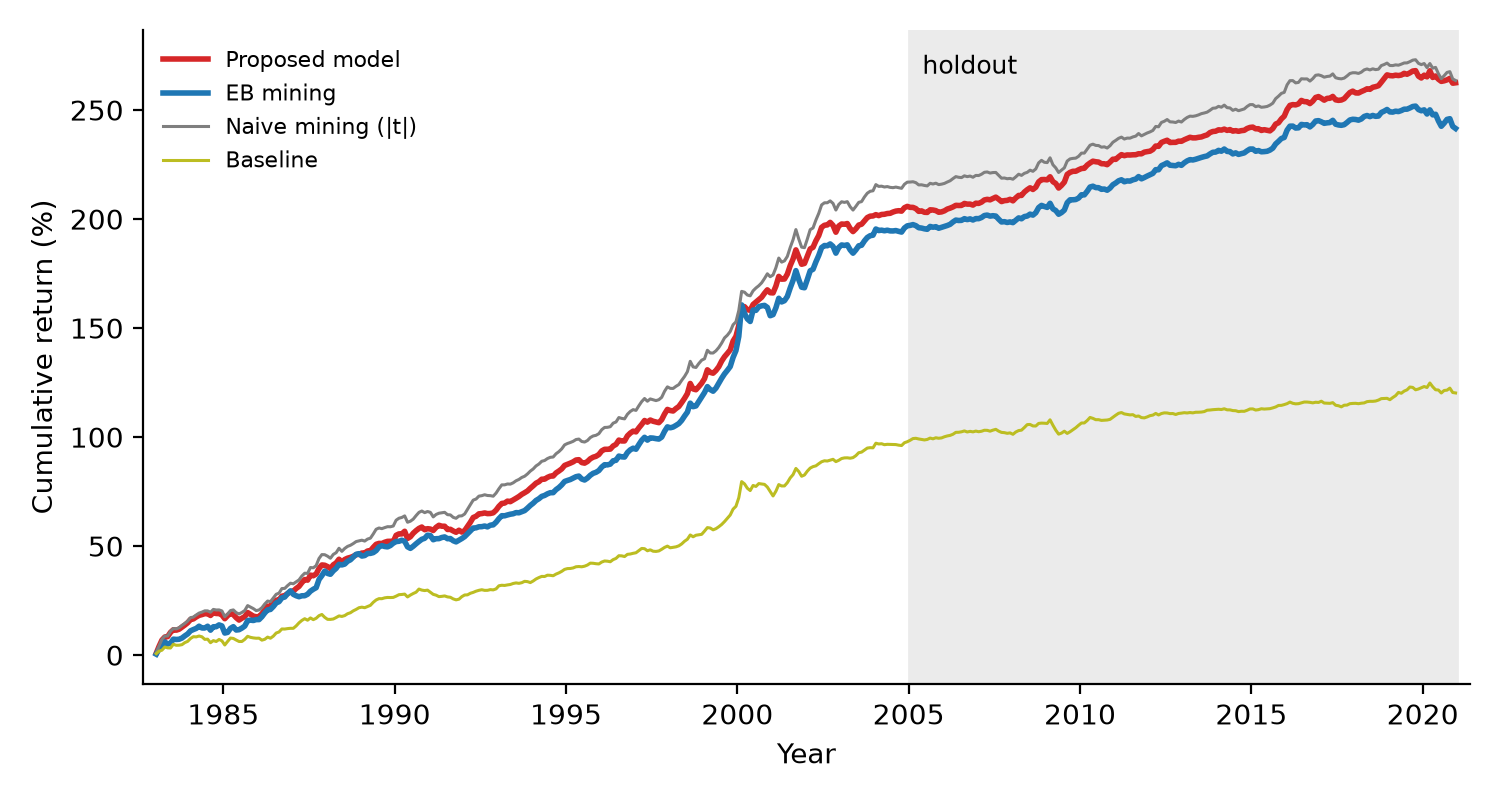
\includegraphics[width=0.9\textwidth]{images/cumret_top1.png}
\caption{Cumulative return (percent) of the top 1\% portfolios. The shaded area is the holdout period.}\label{fig:cumret}
\end{figure}

\subsubsection{Year-by-year performance}
The proposed model does not dominate year by year. Its calendar-year return exceeds that of EB mining in only 21 of the 38 years (13 of 22 in the development period and 8 of 16 in the holdout period), and both methods have a positive return in 33 years. The difference arises in the bad years. The worst calendar-year return is $-2.5\%$ for the proposed model (2005) against $-8.1\%$ for EB mining (2020), and the maximum drawdown of the cumulative return is 6.6 percentage points against 10.3. In the holdout period, the standard deviation of calendar-year returns is 3.5\% against 4.1\%, while in the development period it is slightly higher (6.0\% against 5.5\%), in line with its higher return.

\subsubsection{Performance stability}
Table \ref{tab:subperiod} splits the sample into four subperiods. The top 1\% Sharpe ratio of the proposed model is higher than that of EB mining in all four, and higher than that of naive mining in the last three. This includes the last subperiod, in which predictability is weakest (0.99 against 0.58).

\begin{table}[h]
\caption{Top 1\% Sharpe ratio by subperiod.}\label{tab:subperiod}%
\small
\begin{tabular}{@{}llcccc@{}}
\toprule
Measure & Method & 1983--1994 & 1995--2004 & 2005--2012 & 2013--2020 \\
\midrule
Sharpe ratio & Naive mining ($|t|$ rule) & 2.26 & 1.89 & 1.03 & 0.66 \\
 & EB mining & 2.00 & 1.52 & 1.11 & 0.58 \\
 & Proposed model & 2.17 & 1.97 & 1.25 & 0.99 \\
\botrule
\end{tabular}
\end{table}

% \subsection{Discussion and limitations}\label{subsec5_4}

% \subsubsection{Interpretation}
% The advantage of the proposed model concentrates in one place: the top of the ranking, and it persists after 2004. This is consistent with its design. The label of Equation \eqref{eq:label} compares strategies within a year, and the ablation of Section \ref{subsec4_3} shows that this label and the pretrained encoder contribute to the result, while it does not distinguish ISAB, the Huber loss or the year weights from run-to-run variation. Selecting strategies with large in-sample returns also selects large sampling error, and EB mining corrects this through shrinkage of the t-stat \cite{chen2025highthroughputassetpricing}. Its forecasts are therefore closer to realized returns in magnitude, which may explain its better calibration and higher development IC. The t-stat already carries most of the information for the top of the ranking, which explains why naive mining performs well, consistent with Proposition 1 of \cite{chen2025highthroughputassetpricing}. The proposed model nonetheless adds to it. Two strategies with the same t-stat can differ in how their returns are distributed over time, and the strategies that only the proposed model selects earn a much higher Sharpe ratio than those that only EB mining selects (Section \ref{subsec5_1}), so the return history may carry additional information.

% \subsubsection{Practical implications}
% % For a data miner who holds the top 1\% (about 257 strategies in a typical year) for 12 months, the proposed model offers a higher return per unit of risk and smaller losses in bad years than EB mining, using only information available in real time. Because it ranks better but estimates return magnitudes worse, it fits the task of choosing which strategies to hold, and not the task of forecasting how much they will earn. The holdout return of the top 1\% portfolio is 3.5\% per year before transaction costs, lower than the development return, so the return after 2004 is modest in size.
% Evaluated with the portfolio tests of \cite{chen2025highthroughputassetpricing}, the proposed model selects a top 1\% portfolio with a higher Sharpe ratio than EB mining in the development period (1.95 against 1.55), the holdout period (1.11 against 0.82) and the full period (1.62 against 1.27), and each difference is statistically significant. Among the four methods compared on the same strategies and years, it has the highest top 1\% Sharpe ratio in the holdout and full periods (tied with naive mining in the development period) and the highest holdout Sharpe ratio at all three portfolio sizes. Its losses in bad years are smaller than those of EB mining. The model also recognizes ticker strategies, which carry no predictability, as noise at the top of its ranking (0.19\% of its top 1\% portfolio, against 43.5\% of the pool), although it shrinks them less than EB mining beyond the top 1\%. The ablation indicates that the pretrained encoder, the PCA compression and the label construction contribute to this result.

% This study makes three contributions. First, we propose a label that expresses future performance in Sharpe ratio units and removes the year mean and the part explained by the absolute t-stat, so that the model learns what the t-stat does not already explain. Second, we integrate pretrained temporal representations, cross-strategy interaction and a robust loss into a forecasting model that is re-estimated every year without look-ahead bias. Third, we evaluate the model against EB mining and naive mining with the portfolio tests of \cite{chen2025highthroughputassetpricing} to identify which model components contribute to predictive performance.

% The results have two key implications. First, historical returns contain predictive information beyond the t-statistics used to rank strategies, and this advantage persists after 2004, when predictability weakens. Second, ranking strategies and estimating expected returns are distinct tasks: although the proposed model improves strategy selection, EB mining remains more accurate in estimating return magnitudes. Therefore, the two approaches may complement rather than replace each other.

% \subsubsection{Limitations}
% % First, the proposed model was selected on the development period after exploring about 60 configurations, so the $p$-values are descriptive and not adjusted for multiple testing. Second, retraining the final configuration gives a lower holdout Sharpe ratio on average (0.84 over three runs, against 0.96 for the stored model), so the stored model may be somewhat better than a typical retraining. Third, our evidence concerns the equal-weighted accounting family, which accounts for most of the top 1\% of EB mining, and the advantage over EB mining is statistically supported only for the top 1\% portfolio; it does not extend to other markets. Fourth, FinCast is pretrained on external data whose periods may overlap with our forecasting years, and we cannot rule out that this gives the model some information about them. Finally, the portfolios are before transaction costs.
% This study has several limitations that suggest directions for future research. First of all, the analysis focuses on a single family of long–short strategies in one market, which may limit the generalizability of the findings. Future work could extend the framework to other strategy families and markets to assess the robustness of its predictive performance. Secondly, although the proposed model improves strategy ranking, it is less accurate than empirical Bayes (EB) mining in estimating return magnitudes. Future research could explore forecast calibration or shrinkage techniques to improve the accuracy of return estimates while preserving the model's ranking ability. Finally, the contributions of individual architectural components remain difficult to distinguish due to variations in experimental results across different runs. Further experiments with multiple random seeds and more systematic ablation studies could provide stronger evidence of their respective contributions.


% The input format for the above table is as follows:

% %%=============================================%%
% %% For presentation purpose, we have included  %%
% %% \bigskip command. Please ignore this.       %%
% %%=============================================%%
% \bigskip
% \begin{verbatim}
% \begin{table}[<placement-specifier>]
% \caption{<table-caption>}\label{<table-label>}%
% \begin{tabular}{@{}llll@{}}
% \toprule
% Column 1 & Column 2 & Column 3 & Column 4\\
% \midrule
% row 1 & data 1 & data 2	 & data 3 \\
% row 2 & data 4 & data 5\footnotemark[1] & data 6 \\
% row 3 & data 7 & data 8	 & data 9\footnotemark[2]\\
% \botrule
% \end{tabular}
% \footnotetext{Source: This is an example of table footnote. 
% This is an example of table footnote.}
% \footnotetext[1]{Example for a first table footnote.
% This is an example of table footnote.}
% \footnotetext[2]{Example for a second table footnote. 
% This is an example of table footnote.}
% \end{table}
% \end{verbatim}
% \bigskip
% %%=============================================%%
% %% For presentation purpose, we have included  %%
% %% \bigskip command. Please ignore this.       %%
% %%=============================================%%

% \begin{table}[h]
% \caption{Example of a lengthy table which is set to full textwidth}\label{tab3}
% \begin{tabular*}{\textwidth}{@{\extracolsep\fill}lcccccc}
% \toprule%
% & \multicolumn{3}{@{}c@{}}{Element 1\footnotemark[1]} & \multicolumn{3}{@{}c@{}}{Element 2\footnotemark[2]} \\\cmidrule{2-4}\cmidrule{5-7}%
% Project & Energy & $\sigma_{calc}$ & $\sigma_{expt}$ & Energy & $\sigma_{calc}$ & $\sigma_{expt}$ \\
% \midrule
% Element 3  & 990 A & 1168 & $1547\pm12$ & 780 A & 1166 & $1239\pm100$\\
% Element 4  & 500 A & 961  & $922\pm10$  & 900 A & 1268 & $1092\pm40$\\
% \botrule
% \end{tabular*}
% \footnotetext{Note: This is an example of table footnote. This is an example of table footnote this is an example of table footnote this is an example of~table footnote this is an example of table footnote.}
% \footnotetext[1]{Example for a first table footnote.}
% \footnotetext[2]{Example for a second table footnote.}
% \end{table}

% In case of double column layout, tables which do not fit in single column width should be set to full text width. For this, you need to use \verb+\begin{table*}+ \verb+...+ \verb+\end{table*}+ instead of \verb+\begin{table}+ \verb+...+ \verb+\end{table}+ environment. Lengthy tables which do not fit in textwidth should be set as rotated table. For this, you need to use \verb+\begin{sidewaystable}+ \verb+...+ \verb+\end{sidewaystable}+ instead of \verb+\begin{table*}+ \verb+...+ \verb+\end{table*}+ environment. This environment puts tables rotated to single column width. For tables rotated to double column width, use \verb+\begin{sidewaystable*}+ \verb+...+ \verb+\end{sidewaystable*}+.

% \begin{sidewaystable}
% \caption{Tables which are too long to fit, should be written using the ``sidewaystable'' environment as shown here}\label{tab3}
% \begin{tabular*}{\textheight}{@{\extracolsep\fill}lcccccc}
% \toprule%
% & \multicolumn{3}{@{}c@{}}{Element 1\footnotemark[1]}& \multicolumn{3}{@{}c@{}}{Element\footnotemark[2]} \\\cmidrule{2-4}\cmidrule{5-7}%
% Projectile & Energy	& $\sigma_{calc}$ & $\sigma_{expt}$ & Energy & $\sigma_{calc}$ & $\sigma_{expt}$ \\
% \midrule
% Element 3 & 990 A & 1168 & $1547\pm12$ & 780 A & 1166 & $1239\pm100$ \\
% Element 4 & 500 A & 961  & $922\pm10$  & 900 A & 1268 & $1092\pm40$ \\
% Element 5 & 990 A & 1168 & $1547\pm12$ & 780 A & 1166 & $1239\pm100$ \\
% Element 6 & 500 A & 961  & $922\pm10$  & 900 A & 1268 & $1092\pm40$ \\
% \botrule
% \end{tabular*}
% \footnotetext{Note: This is an example of table footnote this is an example of table footnote this is an example of table footnote this is an example of~table footnote this is an example of table footnote.}
% \footnotetext[1]{This is an example of table footnote.}
% \end{sidewaystable}
% \FloatBarrier



% \section{Conclusion}\label{sec6}

% As per the \LaTeX\ standards you need to use eps images for \LaTeX\ compilation and \verb+pdf/jpg/png+ images for \verb+PDFLaTeX+ compilation. This is one of the major difference between \LaTeX\ and \verb+PDFLaTeX+. Each image should be from a single input .eps/vector image file. Avoid using subfigures. The command for inserting images for \LaTeX\ and \verb+PDFLaTeX+ can be generalized. The package used to insert images in \verb+LaTeX/PDFLaTeX+ is the graphicx package. Figures can be inserted via the normal figure environment as shown in the below example:

% %%=============================================%%
% %% For presentation purpose, we have included  %%
% %% \bigskip command. Please ignore this.       %%
% %%=============================================%%
% \bigskip
% \begin{verbatim}
% \begin{figure}[<placement-specifier>]
% \centering
% \includegraphics{<eps-file>}
% \caption{<figure-caption>}\label{<figure-label>}
% \end{figure}
% \end{verbatim}
% \bigskip
% %%=============================================%%
% %% For presentation purpose, we have included  %%
% %% \bigskip command. Please ignore this.       %%
% %%=============================================%%

% \begin{figure}[h]
% \centering
% 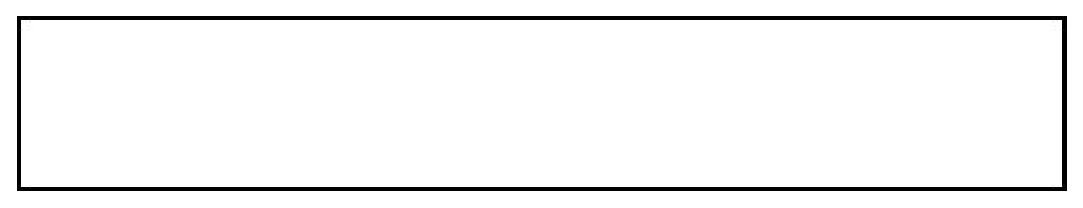
\includegraphics[width=0.9\textwidth]{fig.eps}
% \caption{This is a widefig. This is an example of long caption this is an example of long caption  this is an example of long caption this is an example of long caption}\label{fig1}
% \end{figure}

% In case of double column layout, the above format puts figure captions/images to single column width. To get spanned images, we need to provide \verb+\begin{figure*}+ \verb+...+ \verb+\end{figure*}+.

% For sample purpose, we have included the width of images in the optional argument of \verb+\includegraphics+ tag. Please ignore this. 
\section{Conclusion}\label{sec6}
Overall, the proposed framework integrates a pretrained FinCast encoder, PCA, Bi-LSTM, and attention mechanisms, leveraging their complementary strengths for stock return prediction. FinCast extracts informative representations from historical financial time series, providing a foundation for downstream prediction. However, these representations may contain redundant dimensions, motivating the use of PCA to reduce dimensionality while retaining the principal sources of variation. Since stock returns exhibit temporal dependencies and potentially nonlinear dynamics, Bi-LSTM captures sequential patterns in both forward and backward directions within the historical input sequence. Furthermore, multi-head self-attention models interactions among temporal segments, while the Induced Set Attention Block (ISAB) aggregates relevant information into a compact context vector. Together, these components enable the model to learn complex patterns from historical strategy performance and improve out-of-sample return prediction.

Empirically, the proposed model achieves a Sharpe ratio of up to 1.95 during the development period (1983–2004) and 1.11 during the holdout period (2005–2020). It outperforms benchmark methods for the top 1\% and top 5\% of strategies across both periods and the full sample, as well as for the top 10\% during the holdout period, demonstrating its potential for out-of-sample return prediction. 

Finally, the proposed method demonstrates the potential of deep learning for return prediction by capturing nonlinear relationships among market factors and adapting to changing market dynamics.

% \subsection{Research summary}
% This study investigated whether the return history of a long-short strategy, and not only its summary statistics, helps to select strategies that will earn returns out of sample. For each year from 1983 to 2020, we forecast the mean return of about 26,000 equal-weighted accounting strategies using only earlier data, the quantity that empirical Bayes (EB) predicts. The proposed model employs a pretrained FinCast encoder to represent the 128-month return sequence, compresses it with PCA, summarizes it with a Bi-LSTM and attention pooling, lets the strategies of the same year interact through an ISAB, and combines the result with the t-stat and mean return. It is trained on a label that removes the year mean and the part explained by the absolute t-stat, with a weighted Huber loss, and it is re-estimated every year.

\section{Practical implications}
Evaluated with the portfolio tests of \cite{chen2025highthroughputassetpricing}, the proposed model selects a top 1\% portfolio with a higher Sharpe ratio than EB mining in the development period (1.95 against 1.55), the holdout period (1.11 against 0.82) and the full period (1.62 against 1.27), and each difference is statistically significant. Among the four methods compared on the same strategies and years, it has the highest top 1\% Sharpe ratio in the holdout and full periods (tied with naive mining in the development period) and the highest holdout Sharpe ratio at all three portfolio sizes. Its losses in bad years are smaller than those of EB mining. The model also recognizes ticker strategies, which carry no predictability, as noise at the top of its ranking (0.19\% of its top 1\% portfolio, against 43.5\% of the pool), although it shrinks them less than EB mining beyond the top 1\%. The ablation indicates that the pretrained encoder, the PCA compression and the label construction contribute to this result.

This study makes three contributions. First, we propose a label that expresses future performance in Sharpe ratio units and removes the year mean and the part explained by the absolute t-stat, so that the model learns what the t-stat does not already explain. Second, we integrate pretrained temporal representations, cross-strategy interaction and a robust loss into a forecasting model that is re-estimated every year without look-ahead bias. Third, we evaluate the model against EB mining and naive mining with the portfolio tests of \cite{chen2025highthroughputassetpricing} to identify which model components contribute to predictive performance.

The results have two key implications. First, historical returns contain predictive information beyond the t-statistics used to rank strategies, and this advantage persists after 2004, when predictability weakens. Second, ranking strategies and estimating expected returns are distinct tasks: although the proposed model improves strategy selection, EB mining remains more accurate in estimating return magnitudes. Therefore, the two approaches may complement rather than replace each other.

\section{Limitations and directions for future research}
This study has several limitations that suggest directions for future research. First of all, the analysis focuses on a single family of long–short strategies in one market, which may limit the generalizability of the findings. Future work could extend the framework to other strategy families and markets to assess the robustness of its predictive performance. Secondly, although the proposed model improves strategy ranking, it is less accurate than empirical Bayes (EB) mining in estimating return magnitudes. Future research could explore forecast calibration or shrinkage techniques to improve the accuracy of return estimates while preserving the model's ranking ability. Finally, the contributions of individual architectural components remain difficult to distinguish due to variations in experimental results across different runs. Further experiments with multiple random seeds and more systematic ablation studies could provide stronger evidence of their respective contributions.


% \section{Algorithms, Program codes and Listings}\label{sec7}

% Packages \verb+algorithm+, \verb+algorithmicx+ and \verb+algpseudocode+ are used for setting algorithms in \LaTeX\ using the format:

% %%=============================================%%
% %% For presentation purpose, we have included  %%
% %% \bigskip command. Please ignore this.       %%
% %%=============================================%%
% \bigskip
% \begin{verbatim}
% \begin{algorithm}
% \caption{<alg-caption>}\label{<alg-label>}
% \begin{algorithmic}[1]
% . . .
% \end{algorithmic}
% \end{algorithm}
% \end{verbatim}
% \bigskip
% %%=============================================%%
% %% For presentation purpose, we have included  %%
% %% \bigskip command. Please ignore this.       %%
% %%=============================================%%

% You may refer above listed package documentations for more details before setting \verb+algorithm+ environment. For program codes, the ``verbatim'' package is required and the command to be used is \verb+\begin{verbatim}+ \verb+...+ \verb+\end{verbatim}+. 

% Similarly, for \verb+listings+, use the \verb+listings+ package. \verb+\begin{lstlisting}+ \verb+...+ \verb+\end{lstlisting}+ is used to set environments similar to \verb+verbatim+ environment. Refer to the \verb+lstlisting+ package documentation for more details.

% A fast exponentiation procedure:

% \lstset{texcl=true,basicstyle=\small\sf,commentstyle=\small\rm,mathescape=true,escapeinside={(*}{*)}}
% \begin{lstlisting}
% begin
%   for $i:=1$ to $10$ step $1$ do
%       expt($2,i$);  
%       newline() od                (*\textrm{Comments will be set flush to the right margin}*)
% where
% proc expt($x,n$) $\equiv$
%   $z:=1$;
%   do if $n=0$ then exit fi;
%      do if odd($n$) then exit fi;                 
%         comment: (*\textrm{This is a comment statement;}*)
%         $n:=n/2$; $x:=x*x$ od;
%      { $n>0$ };
%      $n:=n-1$; $z:=z*x$ od;
%   print($z$). 
% end
% \end{lstlisting}

% \begin{algorithm}
% \caption{Calculate $y = x^n$}\label{algo1}
% \begin{algorithmic}[1]
% \Require $n \geq 0 \vee x \neq 0$
% \Ensure $y = x^n$ 
% \State $y \Leftarrow 1$
% \If{$n < 0$}\label{algln2}
%         \State $X \Leftarrow 1 / x$
%         \State $N \Leftarrow -n$
% \Else
%         \State $X \Leftarrow x$
%         \State $N \Leftarrow n$
% \EndIf
% \While{$N \neq 0$}
%         \If{$N$ is even}
%             \State $X \Leftarrow X \times X$
%             \State $N \Leftarrow N / 2$
%         \Else[$N$ is odd]
%             \State $y \Leftarrow y \times X$
%             \State $N \Leftarrow N - 1$
%         \EndIf
% \EndWhile
% \end{algorithmic}
% \end{algorithm}

% %%=============================================%%
% %% For presentation purpose, we have included  %%
% %% \bigskip command. Please ignore this.       %%
% %%=============================================%%
% \bigskip
% \begin{minipage}{\hsize}%
% \lstset{frame=single,framexleftmargin=-1pt,framexrightmargin=-17pt,framesep=12pt,linewidth=0.98\textwidth,language=pascal}% Set your language (you can change the language for each code-block optionally)
% %%% Start your code-block
% \begin{lstlisting}
% for i:=maxint to 0 do
% begin
% { do nothing }
% end;
% Write('Case insensitive ');
% Write('Pascal keywords.');
% \end{lstlisting}
% \end{minipage}

% \section{Cross referencing}\label{sec8}

% Environments such as figure, table, equation and align can have a label
% declared via the \verb+\label{#label}+ command. For figures and table
% environments use the \verb+\label{}+ command inside or just
% below the \verb+\caption{}+ command. You can then use the
% \verb+\ref{#label}+ command to cross-reference them. As an example, consider
% the label declared for Figure~\ref{fig1} which is
% \verb+\label{fig1}+. To cross-reference it, use the command 
% \verb+Figure \ref{fig1}+, for which it comes up as
% ``Figure~\ref{fig1}''. 

% To reference line numbers in an algorithm, consider the label declared for the line number 2 of Algorithm~\ref{algo1} is \verb+\label{algln2}+. To cross-reference it, use the command \verb+\ref{algln2}+ for which it comes up as line~\ref{algln2} of Algorithm~\ref{algo1}.

% \subsection{Details on reference citations}\label{subsec7}

% Standard \LaTeX\ permits only numerical citations. To support both numerical and author-year citations this template uses \verb+natbib+ \LaTeX\ package. For style guidance please refer to the template user manual.

% %Here is an example for \verb+\cite{...}+: \cite{bib1}. Another example for \verb+\citep{...}+: \citep{bib2}. For author-year citation mode, \verb+\cite{...}+ prints Jones et al. (1990) and \verb+\citep{...}+ prints (Jones et al., 1990).

% %All cited bib entries are printed at the end of this article: \cite{bib3}, \cite{bib4}, \cite{bib5}, \cite{bib6}, \cite{bib7}, \cite{bib8}, \cite{bib9}, \cite{bib10}, \cite{bib11}, \cite{bib12} and \cite{bib13}.

% \section{Examples for theorem like environments}\label{sec10}

% For theorem like environments, we require \verb+amsthm+ package. There are three types of predefined theorem styles exists---\verb+thmstyleone+, \verb+thmstyletwo+ and \verb+thmstylethree+ 

% %%=============================================%%
% %% For presentation purpose, we have included  %%
% %% \bigskip command. Please ignore this.       %%
% %%=============================================%%
% \bigskip
% \begin{tabular}{|l|p{19pc}|}
% \hline
% \verb+thmstyleone+ & Numbered, theorem head in bold font and theorem text in italic style \\\hline
% \verb+thmstyletwo+ & Numbered, theorem head in roman font and theorem text in italic style \\\hline
% \verb+thmstylethree+ & Numbered, theorem head in bold font and theorem text in roman style \\\hline
% \end{tabular}
% \bigskip
% %%=============================================%%
% %% For presentation purpose, we have included  %%
% %% \bigskip command. Please ignore this.       %%
% %%=============================================%%

% For mathematics journals, theorem styles can be included as shown in the following examples:

% \begin{theorem}[Theorem subhead]\label{thm1}
% Example theorem text. Example theorem text. Example theorem text. Example theorem text. Example theorem text. 
% Example theorem text. Example theorem text. Example theorem text. Example theorem text. Example theorem text. 
% Example theorem text. 
% \end{theorem}

% Sample body text. Sample body text. Sample body text. Sample body text. Sample body text. Sample body text. Sample body text. Sample body text.

% \begin{proposition}
% Example proposition text. Example proposition text. Example proposition text. Example proposition text. Example proposition text. 
% Example proposition text. Example proposition text. Example proposition text. Example proposition text. Example proposition text. 
% \end{proposition}

% Sample body text. Sample body text. Sample body text. Sample body text. Sample body text. Sample body text. Sample body text. Sample body text.

% \begin{example}
% Phasellus adipiscing semper elit. Proin fermentum massa
% ac quam. Sed diam turpis, molestie vitae, placerat a, molestie nec, leo. Maecenas lacinia. Nam ipsum ligula, eleifend
% at, accumsan nec, suscipit a, ipsum. Morbi blandit ligula feugiat magna. Nunc eleifend consequat lorem. 
% \end{example}

% Sample body text. Sample body text. Sample body text. Sample body text. Sample body text. Sample body text. Sample body text. Sample body text.

% \begin{remark}
% Phasellus adipiscing semper elit. Proin fermentum massa
% ac quam. Sed diam turpis, molestie vitae, placerat a, molestie nec, leo. Maecenas lacinia. Nam ipsum ligula, eleifend
% at, accumsan nec, suscipit a, ipsum. Morbi blandit ligula feugiat magna. Nunc eleifend consequat lorem. 
% \end{remark}

% Sample body text. Sample body text. Sample body text. Sample body text. Sample body text. Sample body text. Sample body text. Sample body text.

% \begin{definition}[Definition sub head]
% Example definition text. Example definition text. Example definition text. Example definition text. Example definition text. Example definition text. Example definition text. Example definition text. 
% \end{definition}

% Additionally a predefined ``proof'' environment is available: \verb+\begin{proof}+ \verb+...+ \verb+\end{proof}+. This prints a ``Proof'' head in italic font style and the ``body text'' in roman font style with an open square at the end of each proof environment. 

% \begin{proof}
% Example for proof text. Example for proof text. Example for proof text. Example for proof text. Example for proof text. Example for proof text. Example for proof text. Example for proof text. Example for proof text. Example for proof text. 
% \end{proof}

% Sample body text. Sample body text. Sample body text. Sample body text. Sample body text. Sample body text. Sample body text. Sample body text.

% \begin{proof}[Proof of Theorem~{\upshape\ref{thm1}}]
% Example for proof text. Example for proof text. Example for proof text. Example for proof text. Example for proof text. Example for proof text. Example for proof text. Example for proof text. Example for proof text. Example for proof text. 
% \end{proof}

% \noindent
% For a quote environment, use \verb+\begin{quote}...\end{quote}+
% \begin{quote}
% Quoted text example. Aliquam porttitor quam a lacus. Praesent vel arcu ut tortor cursus volutpat. In vitae pede quis diam bibendum placerat. Fusce elementum
% convallis neque. Sed dolor orci, scelerisque ac, dapibus nec, ultricies ut, mi. Duis nec dui quis leo sagittis commodo.
% \end{quote}

% Sample body text. Sample body text. Sample body text. Sample body text. Sample body text (refer Figure~\ref{fig1}). Sample body text. Sample body text. Sample body text (refer Table~\ref{tab3}). 

% \section{Methods}\label{sec11}

% Topical subheadings are allowed. Authors must ensure that their Methods section includes adequate experimental and characterization data necessary for others in the field to reproduce their work. Authors are encouraged to include RIIDs where appropriate. 

% \textbf{Ethical approval declarations} (only required where applicable) Any article reporting experiment/s carried out on (i)~live vertebrate (or higher invertebrates), (ii)~humans or (iii)~human samples must include an unambiguous statement within the methods section that meets the following requirements: 

% \begin{enumerate}[1.]
% \item Approval: a statement which confirms that all experimental protocols were approved by a named institutional and/or licensing committee. Please identify the approving body in the methods section

% \item Accordance: a statement explicitly saying that the methods were carried out in accordance with the relevant guidelines and regulations

% \item Informed consent (for experiments involving humans or human tissue samples): include a statement confirming that informed consent was obtained from all participants and/or their legal guardian/s
% \end{enumerate}

% If your manuscript includes potentially identifying patient/participant information, or if it describes human transplantation research, or if it reports results of a clinical trial then  additional information will be required. Please visit (\url{https://www.nature.com/nature-research/editorial-policies}) for Nature Portfolio journals, (\url{https://www.springer.com/gp/authors-editors/journal-author/journal-author-helpdesk/publishing-ethics/14214}) for Springer Nature journals, or (\url{https://www.biomedcentral.com/getpublished/editorial-policies\#ethics+and+consent}) for BMC.

% \section{Discussion}\label{sec12}

% Discussions should be brief and focused. In some disciplines use of Discussion or `Conclusion' is interchangeable. It is not mandatory to use both. Some journals prefer a section `Results and Discussion' followed by a section `Conclusion'. Please refer to Journal-level guidance for any specific requirements. 

% \section{Conclusion}\label{sec13}

% Conclusions may be used to restate your hypothesis or research question, restate your major findings, explain the relevance and the added value of your work, highlight any limitations of your study, describe future directions for research and recommendations. 

% In some disciplines use of Discussion or 'Conclusion' is interchangeable. It is not mandatory to use both. Please refer to Journal-level guidance for any specific requirements. 

% \backmatter

% \bmhead{Supplementary information}

% If your article has accompanying supplementary file/s please state so here. 

% Authors reporting data from electrophoretic gels and blots should supply the full unprocessed scans for key as part of their Supplementary information. This may be requested by the editorial team/s if it is missing.

% Please refer to Journal-level guidance for any specific requirements.

\bmhead{Acknowledgements}

Acknowledgements are not compulsory. Where included they should be brief. Grant or contribution numbers may be acknowledged.

Please refer to Journal-level guidance for any specific requirements.

\section*{Declarations}

Some journals require declarations to be submitted in a standardised format. Please check the Instructions for Authors of the journal to which you are submitting to see if you need to complete this section. If yes, your manuscript must contain the following sections under the heading `Declarations':

\begin{itemize}
\item Funding
\item Conflict of interest/Competing interests (check journal-specific guidelines for which heading to use)
\item Ethics approval and consent to participate
\item Consent for publication
\item Data availability 
\item Materials availability
\item Code availability 
\item Author contribution
\end{itemize}

\noindent
If any of the sections are not relevant to your manuscript, please include the heading and write `Not applicable' for that section. 

%%===================================================%%
%% For presentation purpose, we have included        %%
%% \bigskip command. Please ignore this.             %%
%%===================================================%%
\bigskip
\begin{flushleft}%
Editorial Policies for:

\bigskip\noindent
Springer journals and proceedings: \url{https://www.springer.com/gp/editorial-policies}

\bigskip\noindent
Nature Portfolio journals: \url{https://www.nature.com/nature-research/editorial-policies}

\bigskip\noindent
\textit{Scientific Reports}: \url{https://www.nature.com/srep/journal-policies/editorial-policies}

\bigskip\noindent
BMC journals: \url{https://www.biomedcentral.com/getpublished/editorial-policies}
\end{flushleft}

\begin{appendices}

\section{Section title of first appendix}\label{secA1}

An appendix contains supplementary information that is not an essential part of the text itself but which may be helpful in providing a more comprehensive understanding of the research problem or it is information that is too cumbersome to be included in the body of the paper.

%%=============================================%%
%% For submissions to Nature Portfolio Journals %%
%% please use the heading ``Extended Data''.   %%
%%=============================================%%

%%=============================================================%%
%% Sample for another appendix section			       %%
%%=============================================================%%

%% \section{Example of another appendix section}\label{secA2}%
%% Appendices may be used for helpful, supporting or essential material that would otherwise 
%% clutter, break up or be distracting to the text. Appendices can consist of sections, figures, 
%% tables and equations etc.

\end{appendices}

%%===========================================================================================%%
%% If you are submitting to one of the Nature Portfolio journals, using the eJP submission   %%
%% system, please include the references within the manuscript file itself. You may do this  %%
%% by copying the reference list from your .bbl file, paste it into the main manuscript .tex %%
%% file, and delete the associated \verb+\bibliography+ commands.                            %%
%%===========================================================================================%%
\clearpage
\bibliography{sn-bibliography}
% common bib file
%% if required, the content of .bbl file can be included here once bbl is generated
%\input sn-article.bbl

\end{document}
